  % its not what learner is best,
% but what tuner is best

% CoGEE results are quirky
% but very quirky

% CoGEE slow. not a good candidate for tuning. we are hyperyhyper parmater.

% on the benefits of hyperparameter optimization for software effort estiamtionhttps://www.sharelatex.com/8956978261xpxppstbtcyp
 
\documentclass[10pt,conference]{IEEEtran}
\usepackage{amssymb}
\setcounter{tocdepth}{3}
\usepackage{cite}

\usepackage{enumitem}
 

\usepackage{rotate}
\usepackage{graphicx}
\usepackage{colortbl}
\usepackage{arydshln}
\usepackage{times}
\usepackage[dvipsnames]{xcolor}
\usepackage{rotating}
\usepackage{makecell} 
\usepackage{tabularx}
\usepackage{booktabs}
\usepackage{wrapfig}
\usepackage{tikz}
\usetikzlibrary{angles}
\usepackage{makecell}
\usepackage{tabu}
\usepackage{multirow}
\newcommand{\bi}{\begin{itemize}}
\newcommand{\ei}{\end{itemize}}
\newcommand{\be}{\begin{enumerate}}
\newcommand{\ee}{\end{enumerate}}
\newcommand{\fig}[1]{Figure~\ref{fig:#1}}
\newcommand{\eq}[1]{Equation~\ref{eq:#1}}
\newcommand{\tion}[1]{\S\ref{sect:#1}}

\usepackage{url}
\newcommand{\keywords}[1]{\par\addvspace\baselineskip
\noindent\keywordname\enspace\ignorespaces#1}
%%% graph
\newcommand{\crule}[3][darkgray]{\textcolor{#1}{\rule{#2}{#3}}}

\newcommand{\dbox}[1] { \crule[black!#1]{0.67cm}{0.4cm} 
\hspace{-0.51cm}\scalebox{1}[1.0]{{\textcolor{black}{{\bf $^{#1}$}}}\hspace{0.1mm}}}


\newcommand{\wbox}[1] { \crule[black!#1]{0.67cm}{0.4cm} 
\hspace{-0.51cm}\scalebox{1}[1.0]{{\textcolor{white}{{\bf $^{#1}$}}}\hspace{0.1mm}}}


\newcommand{\quart}[4]{
\begin{picture}(100,6)%1
    {
        \color{black}
        \put(#3,3)
        {\circle*{4}}
        \put(#1,3)
        {\line(1,0){#2}}
    }
\end{picture}
}

\newcommand{\ofr} {
{\textit{out-of-range}}
}


\usepackage[framemethod=tikz]{mdframed}
\usetikzlibrary{shadows}
\usepackage{graphics}
\newmdenv[
tikzsetting= {fill=gray!10},
linewidth=1pt,
roundcorner=2pt, 
shadow=false
]{myshadowbox}

\newenvironment{result}[2]
{\begin{myshadowbox}\textbf{\textit{\underline{Lesson#1:}}} #2}{ 
\end{myshadowbox}}
    
\newcommand{\nm}[1]{\hline\multicolumn{1}{c}{\cellcolor{black} { {\bf \textcolor{white}{#1}}}}}
%\pdfoutput=1





\begin{document}

% \begin{center}
%   {\Large\bfseries\boldmath
%  Why Software Effort Estimation Needs SBSE}\\~\\
%  \normalsize{(A submission to SSBSE'18; author list blinded for review.)}
% \end{center}
\pagestyle{plain}
\thispagestyle{empty}
\title{Hyperparameter Optimization  for    Effort Estimation}
% \author{\IEEEauthorblockN{
% Tianpei Xia, Jianfeng Chen, George Mathew, Xipeng Shen, Tim Menzies}
% \IEEEauthorblockA{Comptuer Science, North Carolina State University, USA}}
% %\institute{blinded}
% \author{\IEEEauthorblockN{Tianpei Xia, Rahul Krishna,
% Jianfeng Chen, George Mathew, Xipeng Shen and
% Tim Menzies}
% \IEEEauthorblockA{Comptuer Science, North Carolina State University, USA\\
% \url{{txia4,rkrish11,jchen37,george2,xshen5}@ncsu.edu, timm@ieee.org}}}

\maketitle

%XXXX effor 
%%%%% dejaeger12  Moeyersoms:2015 grid search
% li09 : ga tun tine weights on columsna dn rows. very slow.
%XXXXX endmeble, no local tuning ekrem09 
%XXXX GA, one data set. singh2012software
%XXXX de, one data set aljahdali2010software
%XXX grid, 3 data sets Song:2013
% 1 data set , bee colony optimization, tuning cocomo IJST70010
% XXX pso, 1 data set Rao14
% CCCC pso, 3 data set Khatibi13
% none of the above compares withr ecent highwater mark publications

% the acuri challenge
% Arcuri2013. just use the defaults



\begin{abstract}
Software analytics has  been widely used in software engineering for many tasks such as 
generating effort estimates for  software projects.
One 
of the ``black arts'' of software analytics is  tunings the  parameters
controlling a  data mining algorithm.
Such hyperparameter optimization has been widely studied in other software analytics domains
(e.g. defect prediction and text mining) but, so far, has not been extensively explored for effort
estimation.
Accordingly, this paper seeks simple, automatic,     effective and fast methods
for finding good  tunings for  automatic software effort estimation.

We introduce a   hyperparameter optimization architecture called
  OIL  (Optimized Inductive Learning). 
  We test OIL  on a wide range of hyperparameter optimizers using  
  data from 945 software projects. After tuning,
  large improvements in effort estimation accuracy were observed
  (measured in terms of the magnitude of the relative error and standardized accuracy).
  
  From those results, we can (a)~recommend
  two
  very fast hyperparamter optimizers 
  and (b)~deprecated many other effort estimation methods.
  Specifically, we will recommend regression trees (CART) tuned by either different evolution or  MOEA/D.
 
   
An important part of this analysis is its reproducability and refutability. All our scripts
and data are on-line. It is hoped that this paper will prompt and enable much more research on better methods
to tune software effort estimators.
\end{abstract}
\begin{IEEEkeywords}
Effort Estimation, Analogy, Evolutionary algorithms
\end{IEEEkeywords}
 

%XXX simplciity
% baselineline: explroe simplex mebfore going compel... or the reusal reaons PLUS we tried going more comple
% and we loastour ability to make conclusoons of those more complex results

\section{Introduction}\label{sect:intro}

This paper explores methods to improve algorithms
for software effort estimation.
This is needed since software  effort estimates   can be 
wildly inaccurate\cite{kemerer1987empirical}. Inadequate or overfull funding can cause a considerable waste of resource and time. For example, NASA canceled its  Check-out Launch Control System project after the initial \$200M estimate was exceeded by another \$200M~\cite{cowing02}. Effort estimations need to be accurate  (if for
no other reason) since many government
organizations demand that the budgets allocated to
large publicly funded projects be double-checked by some estimation model~\cite{MenziesNeg:2017}.  
Non-algorithm techniques that rely on human judgment~\cite{jorgensen2004review} are much harder to  
audit or 
dispute (e.g.,  when the estimate is generated by a senior colleague but disputed by others). 

Sarro et al.~\cite{sarro2016multi} assert that effort  estimation  is  a  critical  activity  for  planning  and
monitoring software project development in order to deliver
the  product  on  time  and  within  budget~\cite{briand2002resource,kocaguneli2011experiences,trendowicz2014software}.   The
competitiveness (and occasionally the survival) of software
organizations depends on their ability to accurately predict
the  effort  required  for  developing  software  systems;  both
over- or under-estimates can negatively affect the outcome
of software projects~\cite{mcconnell2006software,mendes2002further,sommerville2010software,trendowicz2014software}



{\em Hyperparameter} optimization  is the automatic tuning
of the control parameters of a data
mining algorithm.
It is well established that  classification tasks like software defect prediction or 
 text classification can be dramatically improved by such tuning~\cite{Fu2016TuningFS,tanti18,thornton2013auto,AGRAWAL2018,agrawal2017better}.
But as discussed below (see  \S\ref{sbse}), the  benefits of     hyperparameter optimization for   effort estimation 
have not been extensively
studied.  Accordingly, this paper investigates hyperparameter optimization using a wide
range of estimation methods and optimization methods, using data from 945 software projects.
 


The results of this investigation are assessed   with respect to recent comments by 
Acuri \& Fraser~\cite{Arcuri2013} on the    value  of hyperparameter optimization.
They caution that to transition such optimizers  to industry, then they need to be {\bf  fast}:
\begin{quote}
{\em To entail technology transfer to industrial practice, {\em parameters} tuning is a task of responsibility of who develops and releases search-based tools.
A practitioner, that wants to use such tools, should not be required to run large tuning phases before being able to apply those tools on (their) problems at hand~\cite{Arcuri2013}.}
\end{quote}
Also,  optimizers must  be {\bf useful}:
\begin{quote}
{\em At least in the context of test data generation, (tuning) does not seem easy to find good settings that significantly outperform   ``default'' {\em values}. ... Using ``default'' {\em values} is a reasonable and justified choice, whereas {\em parameters} tuning is a long and expensive process that might or might not pay off in the end~\cite{Arcuri2013}.}
\end{quote}
The experiments of this paper show that,  contrary to Acuri \& Fraser's experiences with test generation,
using the defaults for effort estimation leads to far worse estimates that using
tunings learned by
hyperparameter optimization.


We will also show that the most effective tunings found in this way
  vary extensively from data set to data set.
This means that  such optimizations have to be repeated for each new data set. Hence, it is important
to reply to  Acuri \& Fraser's concerns about parameters tuning being
``a long and expensive process''. Certainly, some of our the methods studied here are  slow and would take  164 hours of CPU time (nearly a week) to terminate. Fortunately, the methods we will recommend
terminate in under 2 hours (on a standard 2GHz desktop machine with 8GB of RAM). 

%XXXX effor 
%%%%% dejaeger12  Moeyersoms:2015 grid search
% li09 : ga tun tine weights on columsna dn rows. very slow.
%XXXXX endmeble, no local tuning ekrem09 
%XXXX GA, one data set. singh2012software
%XXXX de, one data set aljahdali2010software
%XXX grid, 3 data sets Song:2013
% 1 data set , bee colony optimization, tuning cocomo IJST70010
% XXX pso, 1 data set Rao14
% CCCC pso, 3 data set Khatibi13
% none of the above compares withr ecent highwater mark publications

% \begin{table*}[!t]
% \caption{CART's parameters.}\label{tbl:cart}
% \footnoteisze
% \begin{center}
% \begin{tabular}{r|c|c|p{3.2in}}


% Parameter & Default & Tuning range & Notes\\\hline 

% max\_feature & None &[0.01,1]& The number of {\em features} to consider when looking for the best split. \\\hline

% max\_depth & None & [1, 12]& The max depth of the tree. \\ \hline

% min\_sample\_split & 2 &[2,20]& The min number of samples required to split an internal node. \\ \hline

% min\_samples\_leaf & 1 & [1,12]&The min number of samples required to be at a leaf node. 

% \end{tabular}  
% \end{center}
% \end{table*}

\begin{table*}[!t]
\centering
\caption{CART's parameters.}\label{tbl:cart}
\begin{tabular}{r|c|c|p{3.2in}}
Parameter          & Default & Tuning Range  & Notes                                                            \\\hline
max\_feature       & None    & {[}0.01, 1{]} & The number of feature to consider when looking for the best split. \\\hline 
max\_depth         & None    & {[}1, 12{]}   & The maximum depth of the tree.                                     \\\hline 
min\_sample\_split & 2       & {[}0, 20{]}   & The minimum number of samples required to split an internal node.  \\\hline 
min\_samples\_leaf & 1       & {[}1, 12{]}   & The minimum number of samples required to be at a leaf node.      
\end{tabular}
\end{table*}





Overall the contributions of this paper are:
\bi
\item An extensible open-source architecture called OIL that supports the experiments of this paper,
as well as extensions to other experiments. OIL makes the results of this paper repeatable and refutable.
\item
To the best of our knowledge, the largest study yet undertaken of hyperparamter optimization and effort estimation. Prior studies in this arena~\cite{dejaeger12,Moeyersoms:2015,li09,ekrem09,singh2012software,aljahdali2010software,Song:2013,IJST70010,Rao14,Khatibi13} suffered  from  numerous  limitations  such  as
restrictive  assumptions  on  the
attributes
used  in  the  data;
limited  exploration  of  the  parameter  space;  testing  on  very
few  data  sets;  using  optimiziers  that  are  deprecated  in  the
literature;  and  not  benchmarking those  results  against
widely used or prominent recent methods.
\item A demonstration that defaults settings are not the best way to perform effort estimation.
\item The identification of two hyperparameter optimizers that are recommended for effort estimation.
 \item The identification of numerous other effort estimation methods that should be deprecated.
\ei
The rest of this paper is structured as follows.
The next section discusses different methods for effort estimation and how to optimize
the parameters of effort estimation methods. This is followed by a description of our data, our experimental
methods, and our results. After that, a discussion section explores open issues with this work. 

Our conclusion will be that  while Acuri \& Fraser's pessimism about hyperparameter optimization  applies to their
test data generation domain, there exists other domains (e.g. effort estimation) where hyperparamter optimization is both fast and useful.
It is hoped that OIL, and the results of  this paper,  will prompt and enable much more research on better methods
to tune software effort estimators.


\section{About Effort Estimation} 
Software effort estimation is the process of predicting the most realistic amount of human effort (usually expressed in terms of hours, days or months of human work) required to plan, design and develop a software project based on the information collected in previous related software projects.
As shown below, effort estimation techniques can be divided   into human-based  and algorithm-based~\cite{teak2012,shepperd2007software}.

\subsection{Human-based Methods}

There  are many human-based estimations methods~\cite{Jorgensen2004} including methods for agile projects such as planning poker~\cite{molokk08} where participants offer anonymous “bids” on the completion time for a project. When bids are widely divergent, factors leading to that disgreement are elaborated and debated. This cycle of bid+discuss repeats until a consensus
is reached.

% It should be noted that  planning poker is
% used to incrementally assess effort for particular tasks in the scrum backlog.
% This is a  different and simpler task than the
% initial
% estimation of software projects. This is an important issue since
% the initial budget allocation may require a significant amount of intra-organizational lobbying between groups with competing concerns (this is particularly true for larger projects). 
% Since it can be challenging to change such initial budget allocations, it is important
% to get the initial estimate as accurate as possible.

For several reasons, this paper does not explore human-based  estimation methods.
Firstly,   it is known that humans rarely update their human-based estimation knowledge
based on feedback from new projects~\cite{jorgensen2009impact}.
Secondly, algorithm-based methods are preferred when   estimate have to be audited or debated
(since the  method is explicit and   available for inspection). 
Thirdly, algorithm-based methods can be run many times (each time applying small mutations to the input data)
to understand the range of possible estimates.
Even very strong
advocates of human-based methods~\cite{jorg2015a} acknowledge that algorithm-based methods are useful for learning
the
uncertainty
about particular estimates.

\subsection{Algorithm-based Methods}

% Software effort estimation has been extensively
% studied in the SE literature:
% \bi
% \item
% J\"orgensen \& Shepperd list    250+ papers
% proposing new methods for project size or effort estimation~\cite{jorgensen2007systematic}. 
% \item
% We list below 6,000+   methods
% just for  analogy-based effort  estimation (a particular kind of algorithm-based estimation method, described  below in more detail).
% \ei
% Given the existence of so many  methods, it is now
% a matter of some debate about which  method is best for a new data set.
% To simplify that task, 
%XXXX need to intro in intro the large number of methds
% Whigham et al. recommend ATLM since, they claim, ``it performs well over a range of different project types and requires no {\em parameters} tuning''. 
% Note that ``no
% {\em parameters} tuning''  is an attractive property since  tuning   can be very slow--
% particularly when using  {\em hyperparameters} optimization and genetic  algorithms. For example,
% this paper studies effort estimation using multiple evolutionary algorithms
% and 10*3-way cross-validation experiment\footnote{10 times, randomized order of  data. Each time, divide the data into three bins. For each  bin, test a model that was trained  from the other   bins.}. Even with
% cloud compute facilities, our experiments   took 16 hours to complete.
%XXX need to mveo this to intro,,someehow

 Whigham et al.'s ATLM method from TOSEM'15 is an example of an algorithm-based automatic effort estimation method~\cite{Whigham:2015}. ATLM is a multiple linear regression model which calculate the effort as $\mathit{effort} = \beta_0 + \sum_i\beta_i\times a_{i} +  \varepsilon_i$,  where $a_i$ are explanatory {\em attributes} and $\varepsilon_i$ are errors to the actual {\em value}. The prediction weights $\beta_i$ are determined using a least square error estimation~\cite{neter1996applied}. Additionally, transformations are applied on the attributes to further minimize the error in the model. In case of categorical attributes the standard contrasts approach of ``dummy variables"~\cite{hardy1993regression} is applied. While, for continuous attributes, transformations such as logarithmic, square root,  or no transformation is employed such that the skewness of the attribute is minimum. It should be noted that, ATLM does not consider relatively complex techniques like using model residuals,  box transformations or step-wise regression (which are standard) when developing a linear regression model. The authors make this decision since they intend ATLM to be a simple baseline model rather than the ``best" model.


Apart from ATLM, there are many more algorithmic estimation methods. Some, such as COCOMO~\cite{boehm1981software}, make assumptions
about the  attributes in the model. For example, COCOMO requires that the
data include 22 specific   attributes such as analyst capability (acap) and software complexity (cplx).  This   attribute
assumptions restrict the number
of data sets that can be processed by studies like this paper. For example,
this study explore 965 projects expressed using a  wide range of  attributes.  If we used COCOMO, we could only access an order of magnitude   fewer projects.

Sarro et al.'s CoGEE~\cite{sarro2016multi} addresses
the problem of  attribute assumptions. CoGEE in a genetic program
that mutates: \[\mathit{effort} = \beta_1 \mathit{op}_1 a_1  ... \beta_{1n} \mathit{op}_{2n-1} a_n  \mathit{op}_{2n} \beta_0\]
where $a_i$ is an {\em attribute} {\em value} for a project,  $\beta_i \in R$ are weighting numbers and
\mbox{$\mathit{op_i}\in \{+,-,*\}$}. Note that while methods like COCOMO require $a_i$ to be from some reserved set, 
CoGEE will accept data with any {\em attributes}.




Another kind of algorithm-based estimation method are regression trees such as   CART~\cite{brieman84}.  
CART is a  tree learner that divides a data set, then recurses
on each split.
If data contains more than {\em min\_sample\_split}, then a split is attempted.
On the other hand, if a split contains no more than {\em min\_samples\_leaf}, then the recursion stops. 
CART finds the attributes whose ranges contain rows with least variance in the number
of defects. If an  attribute ranges $r_i$ is found in 
$n_i$ rows each with an effort  variance of $v_i$, then CART seeks the  attribute with a split that most
minimizes $\sum_i \left(\sqrt{v_i}\times n_i/(\sum_i n_i)\right)$.
For more details on the CART {\em parameters}, see Table~\ref{tbl:cart}.





%It can be generated using an algorithmic approach or via induced prediction systems. In the former, a senior expert proposes a general model, then use domain data to tune that model to specific projects. For example, a model named COCOMO created by Boehm~\cite{boehm1981software} hypothesized that the software development effort was exponential on LOC and linear on 15 effort multipliers such as analyst capability, product complexity, etc. Boehm defined a local calibration procedure to tune the COCOMO model to local data. If the available local training data does not conform to the requirements of a pre-defined algorithmic model like COCOMO, then the later one, induced prediction systems are useful. There are many induction methods, including linear regression, neural nets, and analogy, etc. However, all of these induction systems require a bias in order to decide what details can be safely ignored. When data violates these assumptions, finding a suitable patch could be difficult without an experienced expert.
 
  



% The results from that study  let us comment on three research questions:
% \bi
% \item XXX
% {\bf RQ1: Can effort estimation ignore SBSE? That is, is tuning avoidable since  just a few options are typically ``best''?} 
% We will find that the ``best'' effort estimation method is highly variable.   That is, tools like OIL are important for
% ensuring that the right estimators are being applied to the current data set.
% \item
% {\bf RQ2: Pragmatically speaking, is SBSE too hard to apply to effort estimation?}
% As shown below, 
% a few dozen evaluations of OIL are enough to  explore  
% configuration options for   effort estimation. That is, it is hardly arduous to apply SBSE to effort
% estimation. Even on a standard single core machine, the median
% time to explore all those options is just  a few minutes.
% \item
% {\bf RQ3: Does SBSE    estimate better than widely-used effort estimation methods?}
% As shown below, the  estimations from OIL perform much  better than  standard effort estimation methods, including   ATLM. 
% \ei


 %~\cite{dejaeger12,Moeyersoms:2015 grid search
% li09 : ga tun tine weights on columsna dn rows. very slow.
%XXXXX endmeble, no local tuning ekrem09 
%XXXX GA, one data set. singh2012software
%XXXX de, one data set aljahdali2010software
%XXX grid, 3 data sets Song:2013
% 1 data set , bee colony optimization, tuning cocomo IJST70010
% XXX pso, 1 data set Rao14
% CCCC pso, 3 data set Khatibi13
% none of the above compares withr ecent highwater mark publications


%~\cite{dejaeger12,Moeyersoms:2015 grid search
% li09 : ga tun tine weights on columsna dn rows. very slow.
%XXXXX endmeble, no local tuning ekrem09 
%XXXX GA, one data set. singh2012software
%XXXX de, one data set aljahdali2010software
%XXX grid, 3 data sets Song:2013
% 1 data set , bee colony optimization, tuning cocomo IJST70010
% XXX pso, 1 data set Rao14
% CCCC pso, 3 data set Khatibi13
% none of the above compares withr ecent highwater mark publications

 
%  their warning
% applies to any software analytics task that dares to propose {\em hyperparameter} optimization. Accordingly, this paper assesses {\em hyperparameter} optimization
% for effort estimation 

% In practice, commissioning an effort estimator on new data takes even more time than stated above. 
% Wolpert's no-free lunch theorems warn that for machine learning~\cite{Wolpert96}, no single method works best on all data sets. Hence, when
% building effort estimators for 
% a new data set, some  {\em commissioning process} is required that tries a range of different algorithms. This is not a
% mere theoretical concern:    researchers report that the ``best'' effort estimator for different
% data sets   varies enormously~\cite{Minku:2011,MINKU20131512,Kocaguneli:2012}.

% Given such  long runtimes, we have found it challenging to make  SBSE attractive to the broader community of  standard developers and business users. 
% To address that challenge, it would be useful to have an example where  SBSE can commission a specific effort estimator for a specific data set, in just a few minutes   on a standard laptop.


% This paper offers such an example. We present a surprising and fortunate result that a very ``CPU-lite'' SBSE
% method  can commission an effort estimator that significantly out-performs
% standard effort estimation methods. Here, by ``out-perform'' we mean that:
% \bi
% \item
% Our estimates have statistically much smaller errors than standard methods;
% \item
% The comissioning time for that estimator is  very fast: median runtime for our ten-way cross-vals is just six minutes on   a   standard
% 8GB,  3GHz  desktop  machine.
% \ei
% Note that our approach is very different to much of the prior research
% on effort estimation and evolutionary algorithms~\cite{BURGESS2001863,879821,5635145,5598118,Lefley:2003:UGP:1756582.1756742,sarro2017adaptive,8255666,shen02a,sarro2016multi,minku2013analysis}. Firstly, that work assumed
% a ``CPU-heavy'' approach whereas we seek a ``CPU-lite'' method. Secondly, we do not defend one particular estimator; instead, our commissioning process selects   a different estimator for each data set  after exploring thousands of possibilities.



% The premise of this paper is that there are {\em too many effort
% estimation methods}. Many of those methods  exhibit
% a ``many roads lead to Rome'' property.
% That is,  when multiple  methods
%  are applied to the same data, many of them have equivalent results. 
%  For such ``many roads'' SE problems, it
%  is unnecessary to explore {\em all} those methods. Rather, it is enough
%  to intelligently sample just a small subset of those methods. 



% Our investigation will address four research questions:
% \bi
% %\item {\bf RQ 1: How to evaluate the performance of our effort estimate method in general?}
% %We use two different measurements methods (MRE and SA) to evaluate the performance of DE tuned ABE approach.
% %\item {\bf RQ 2: How do we compare our methods with established baseline (like Whigham's ATLM) in software literature?}
% %We use plot graph to show the MRE/SA difference between baseline and our method. 
% \item {\bf RQ 1: Does OIL tuning perform better than   random sampling?}
% Methodologically,  SBSE methods should be compared
% against  uninformed random search~\cite{nair18}.
% \item {\bf RQ 2: Are the required runtimes for   SBSE  effort estimation very  slow?}
% This questions checks the overhead for applying SBSE to effort estimation.
% %\item {\bf RQ 5: Can SBSE simplify effort estimation?}
% %The results of our experiments suggest that DE tuning simplify effort estimation by proving better performance within same or less running time.
% \item {\bf RQ 3: Are    OIL's results better
% than accepted practice 
% in effort estimation?}
% For this research question, we compare our results against ABE0
% and ATLM, two standard
% methods in effort estimation.
% \item {\bf RQ 4: Do different datasets require different tunings?}
% If  all datasets required the same tunings, then OIL would  be superfluous since there would be no
% need to apply SBSE to every new data set. 
% \ei
% The rest of this paper is structured as follows.  Section~\tion{background} describes background and related work. How important the effort estimation is and what kinds of techniques have been used. Explains the concept of ABE and introduces how OIL
% to explore different configurations of effort estimators. Section~\tion{study} describes the effort dataset used by this paper, performance metrics and benchmark of the experiments. Section~\tion{results} presents the results of experiments and answers the above questions. Section~\tion{threats} discusses the potential issues and limitations of the our methods. 
% Section~\tion{discussion} and
% Section~\tion{conclusion} discuss our results and propose   future work.
 
%  Note that this is the first paper to introduce OIL. Also,  the scripts and data used in this paper are available on-line at (url hidden for double-blind review).
 


Yet another algorithm-based estimator are the 
analogy-based Estimation (ABE) methods advocted by Shepperd and Schofield~\cite{shepperd1997estimating}. ABE is widely-used~\cite{7194627,Kocaguneli2015,7426628,6092574,MenziesNeg:2017}, in many forms.
We  say that  ``ABE0'' is the standard  form  seen in the literature
and ``ABEN'' are the 6,000+ variants of ABE  defined below. 
The general form of ABE (which applies to  ABE0 or ABEN) is
to first form a table of rows of past projects. The {\em columns} of this table are composed of independent variables (the {\em features} that define projects) and one dependent {\em feature} (project  effort).
From this table, we   what  similar projects (analogies) to use from the training set when examining a new test instance.
For each test instance, ABE then selects   $k$ analogies out of the training set.
Analogies are selected via   a {\em similarity measure}. 
Before calculating similarity,  ABE normalizes   numerics  min..max to 0..1 (so all numerics   get equal chance to influence the dependent). 
Them ABE uses {\em feature} weighting to reduce the influence of less informative {\em features}.
Finally, some  {\em adaption strategy} is applied  return some combination of  the dependent effort {\em values} seen in  the $k$ nearest analogies.

For  details on ABE0 and ABEN, see \fig{featuretree} \& Table~\ref{tbl:aben}. 





\begin{table}[!t]
\caption{Variations on analogy. 
 Visualized in
\fig{featuretree}.}\label{tbl:aben}

\begin{tabular}{|p{.94\linewidth}|}\hline

\begin{itemize}[leftmargin=0.1in]
\item
To measure    similarity between  $x,y$, 
ABE uses $\sqrt{\sum_{i=1}^n w_i(x_i-y_i)^2}$ where  $w_i$ corresponds to {\em feature} weights applied to independent {\em features}. ABEO0 uses a uniform weighting where $w_i=1$.
ABE0's {\em adaptation strategy} is to return the  effort   of the nearest $k=1$   item.
\item
{\em Two ways to find training subsets}:
(a) Remove nothing: Usually, effort estimators use all training projects~\cite{chang1974finding}. Our ABE0 is using this variant;
(b) Outlier methods: prune training projects with (say) suspiciously large {\em values}~\cite{keung2008analogy}. Typically, this removes a small percentage of the training data.
\item
{\em Eight ways to make feature weighting}:
Li {\it et al.}~\cite{li2009study} and Hall and Holmes~\cite{hall2003benchmarking} review 8 different {\em feature} weighting schemes.
\item
{\em Three ways to discretize} (summarize numeric ranges into a few bins):
Some {\em feature} weighting schemes require an initial discretization of continuous {\em columns}. There are many discretization policies in the literature, including:
(1)~equal frequency,
(2)~equal width, 
% (4)PKID~\cite{yang2002comparative},
(3)~do nothing.
\item
{\em Six ways to choose similarity measurements:}
Mendes {\it et al.}~\cite{mendes2003comparative} discuss three similarity measures, including the weighted Euclidean measure described above, an unweighted variant (where $w_i$ = 1), and a ``maximum distance'' measure that focuses on the single {\em feature} that maximizes interproject distance. Frank {\it et al.}~\cite{frank2002locally} use a triangular distribution that sets to the weight to zero after the distance is more than ``k'' neighbors away from the test instance. A fifth and sixth similarity measure are the Minkowski distance measure used in~\cite{angelis2000simulation} and the mean {\em value} of the ranking of each project {\em feature} used in~\cite{walkerden1999empirical}.
\item
{\em Four ways for adaption mechanisms:} 
(1)~median effort {\em value},
(2)~mean dependent {\em value},
(3)~summarize the adaptations via a second learner (e.g., linear regression)~\cite{li2009study,menzies2006selecting,baker2007hybrid,quinlan1992learning},
(4)~weighted mean~\cite{mendes2003comparative}.
\item
{\em Six ways to select analogies:}
Analogy selectors  are  fixed or dynamic~\cite{teak2012}. Fixed methods use $k\in\{1,2,3,4,5\}$
nearest neighbors
while  dynamic methods use the training set to find which $1 \le k \le N-1$ is best for   $N$ examples.
\end{itemize}
\\\hline
\end{tabular}
\end{table}

\begin{figure*}[!t]
\centerline{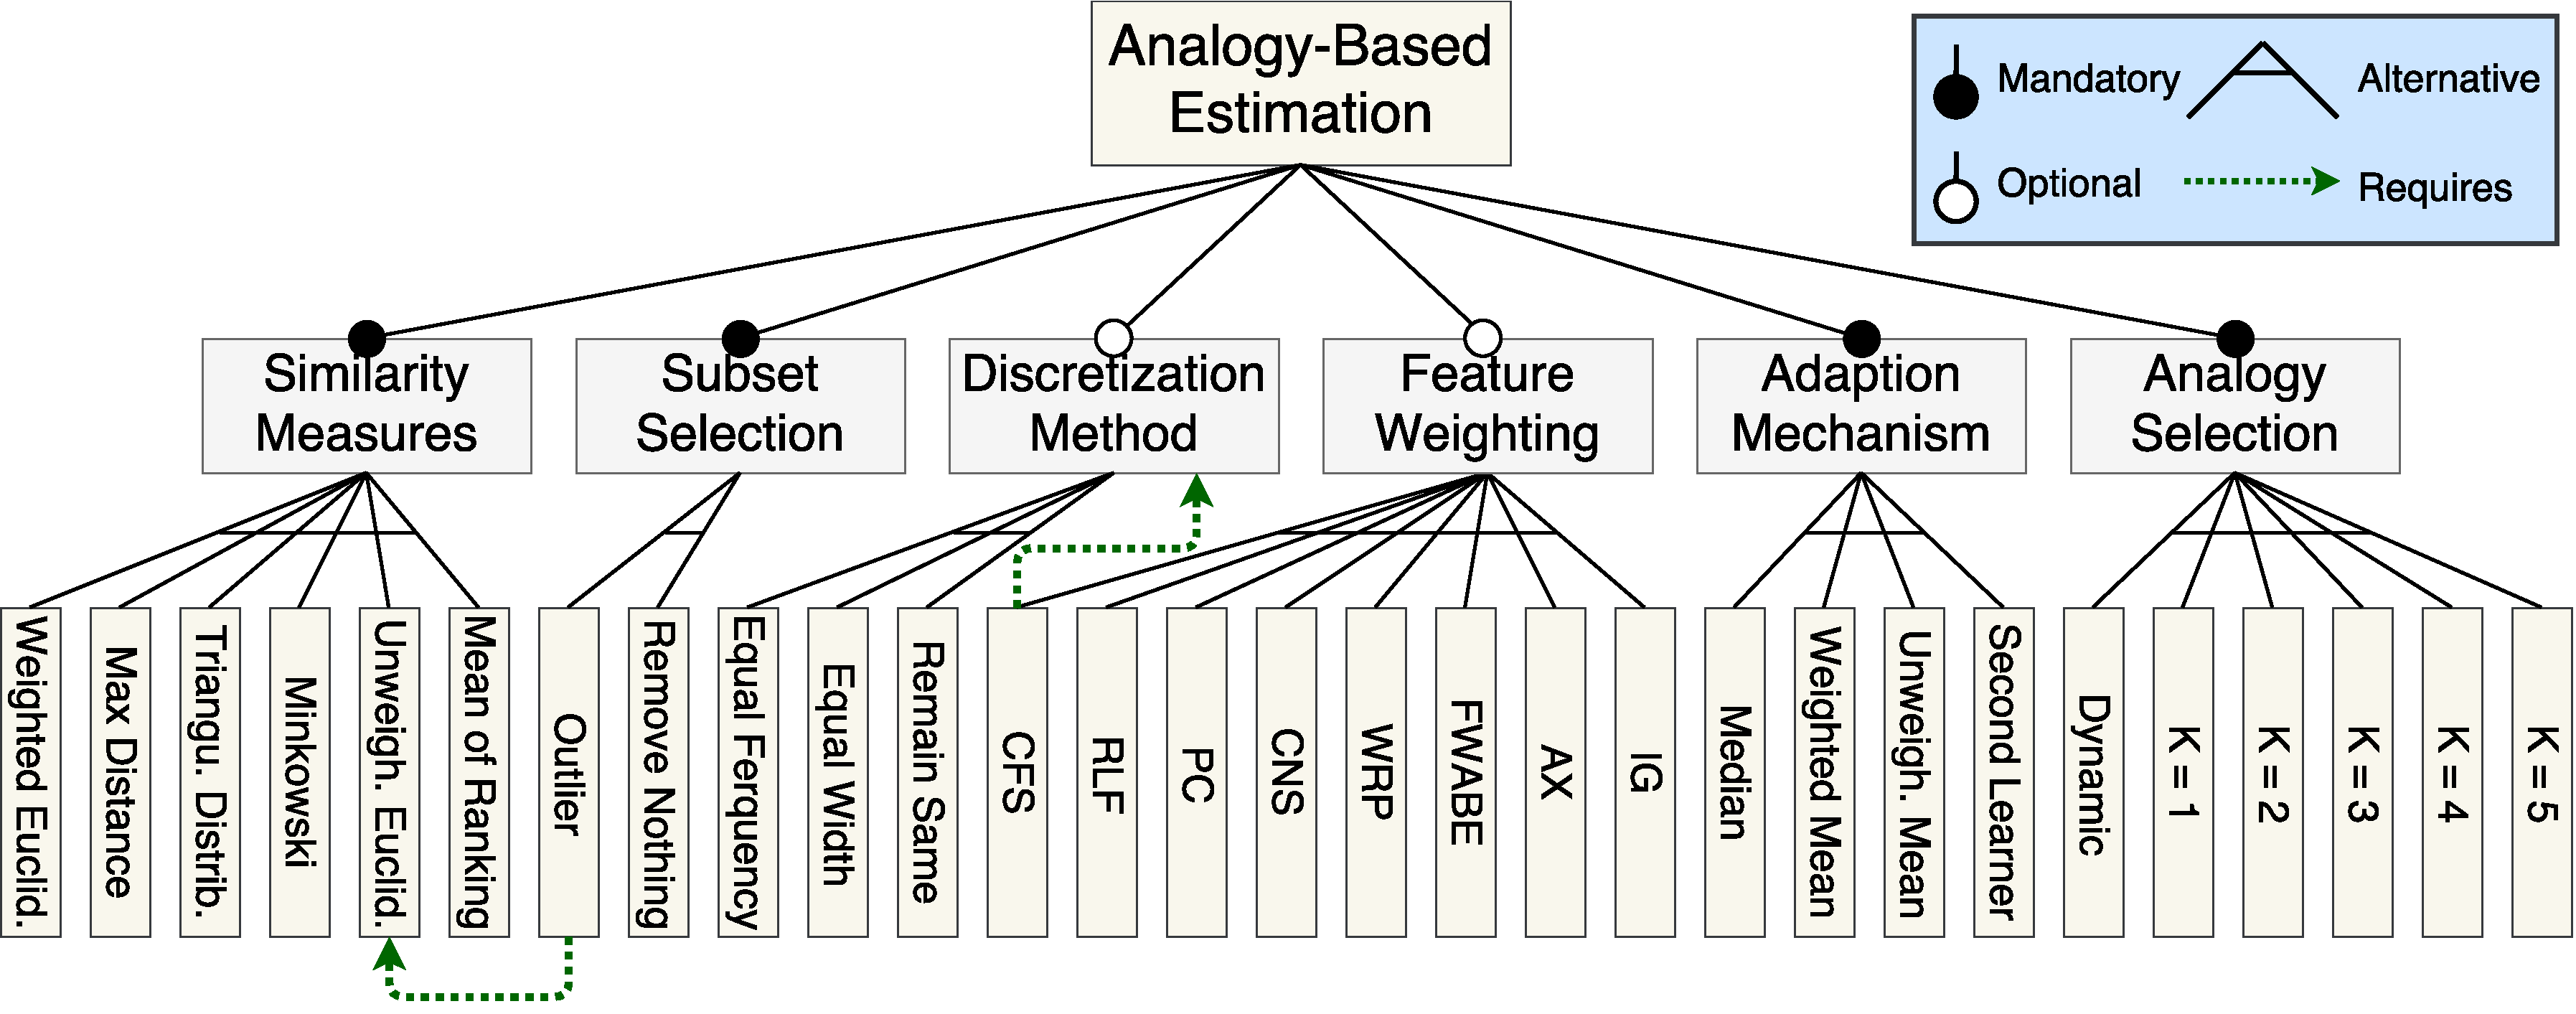
\includegraphics[width=.7\textwidth]{FTM.pdf}}
\caption{OIL's feature model of the space of machine learning options for ABEN.  In this model, $\mathit{Subset Selection}$, $\mathit{Similarity}$, $\mathit{Adaption Mechanism}$ and $\mathit{Analogy Selection}$ are the mandatory {\em features}, while the $\mathit{Feature Weighting}$ and $\mathit{Discretization Method}$ {\em features} are optimal. To avoid making the graph too complex, some cross-tree constrains are not presented.}    
\label{fig:featuretree}
\end{figure*}


\subsection{Effort Estimation and  Hyperparameter Optimization}\label{sbse}


Note that we do \underline{{\em not}} claim that the above represents all methods for  effort estimation. Rather, we  say that (a)~all the above are either prominent in the literature or widely used; and (b)~anyone  with knowledge of  the current effort estimation 
literature would be tempted to try some of the above.

While the above list is incomplete, it is certainly very long. Consider, for example, just the ABEN
variants documented in Table~\ref{tbl:aben}. There are 
$2\times 8\times 3\times 6\times 4\times 6=6,912$ such variants.  Some   can be ignored;
e.g. at $k=1$,     adaptation mechanisms return the same result, so they are not necessary. Also, not all  {\em feature} weighting techniques use discretization. But even after those discards, there are still thousands of possibilities. 

Given the space to exploration is so large, some researchers have offered automatic support for that exploration.
Some of that prior work suffered from being applied to limited data~\cite{li09} or optimizing
with algorithms that are not representative of  the state-of-the-art in multi-objective optimization~\cite{li09}.

Another issue with prior work is that researchers use methods that are widely deprecated in the literature. 
For example,  grid search~\cite{dejaeger12,Song:2013}  is a set of
nested for-loops that iterate over  a range of options.
Grid search is very slow and, due to  the size of the increment in each for-loop, can miss important settings~\cite{Bergstra:2012}.

Other researchers assume that the effort model is a specific parametric form (e.g. the COCOMO equation)
and propose mutation methods to adjust the parameters of that equation~\cite{aljahdali2010software,Moeyersoms:2015,singh2012software,IJST70010,Rao14}. As mentioned above, this approach is
hard to test since there are very few data sets using the   pre-specified COCOMO attributes. 

Further, all that prior work needs to be revisited given the existance of recent and very prominent
methods; i.e.  ATLM and CoGEE system.


Accordingly, this paper conducts a  more thorough investigation of   hyperparameter  optimization for effort estimation. 
In our study:
\bi
\item
We  use methods with no   data
feature assumptions (i.e. no COCOMO data);
\item
That
 vary
many   parameters (6000+ combinations);
\item
That also  tests  results   on 9 different sources with data on 965 software projects; 
\item
Which  uses optimizers   representative of the  state-of-the-art 
(NSGA-II~\cite{deb02}, MOEA/D~\cite{Zhang07}, DE~\cite{storn1997differential});
\item
And which 
benchmark results 
against  prominent methods
  ATLM method from TOSEM'15~\cite{Whigham:2015}; and CoGEE from ICSE'16~\cite{sarro2016multi}.
\ei
One issue we found with CoGEE was that there was no reference implementation 
available for the CoGEE   home page\footnote{www0.cs.ucl.ac.uk/staff/F.Sarro/projects/CoGEE}. Hence, we   built our own   which
raises the possibility that our ``CoGEE'' is different to that reported at ICSE'16. One area
where this might be true was in the area of feature selection. We use much of the same
data as Sarro et al. but   they report that they used fewer columns that was is available in that  data.
This suggests that CoGEE comes with an undocumented feature selection component. 


\pdfoutput=1
\begin{table*}[t!]
\caption{Descriptive Statistics of the Datasets}\label{table:dataset}
\renewcommand{\baselinestretch}{0.75} 
\centering
\begin{tabular}{cc}
\scriptsize
\begin{tabular}{|c|l|rrrr|}
    \hline
      & feature & min  & max & mean & std\\
   \hline

%%%%%%%%%%%%%%%%%%%%%%%%%%%%%%%%%%%%%%%%%%%%%%%%%%%%%%%%%%%%%%%%%%%%

\multirow{7}{*}{\begin{sideways}kemerer\end{sideways}}
& Langu. & 1 & 3 & 1.2 & 0.6\\
& Hdware & 1 & 6 & 2.3 & 1.7\\
& Duration & 5 & 31 & 14.3 & 7.5\\
& KSLOC & 39 & 450 & 186.6 & 136.8\\
& AdjFP & 100 & 2307 & 999.1 & 589.6\\
& RAWFP & 97 & 2284 & 993.9 & 597.4\\
& Effort & 23 & 1107 & 219.2 & 263.1\\
\hline
\multirow{8}{*}{\begin{sideways}albrecht\end{sideways}}
& Input & 7 & 193 & 40.2 & 36.9\\
& Output & 12 & 150 & 47.2 & 35.2\\
& Inquiry & 0 & 75 & 16.9 & 19.3\\
& File & 3 & 60 & 17.4 & 15.5\\
& FPAdj & 1 & 1 & 1.0 & 0.1\\
& RawFPs & 190 & 1902 & 638.5 & 452.7\\
& AdjFP & 199 & 1902 & 647.6 & 488.0\\
& Effort & 0 & 105 & 21.9 & 28.4\\
\hline
\multirow{12}{*}{\begin{sideways}isbsg10\end{sideways}}
% & Data\_Quality & 1 & 2 & 1.2 & 0.4\\
& UFP & 1 & 2 & 1.2 & 0.4\\
& IS & 1 & 10 & 3.2 & 3.0\\
& DP & 1 & 5 & 2.6 & 1.1\\
& LT & 1 & 3 & 1.6 & 0.8\\
& PPL & 1 & 14 & 5.1 & 4.1\\
& CA & 1 & 2 & 1.1 & 0.3\\
& FS & 44 & 1371 & 343.8 & 304.2\\
& RS & 1 & 4 & 1.7 & 0.9\\
% & Recording\_Method & 1 & 4 & 1.8 & 1.0\\
& FPS & 1 & 5 & 3.5 & 0.7\\
& Effort & 87 & 14453 & 2959 & 3518\\
\hline
\multirow{8}{*}{\begin{sideways}finnish\end{sideways}}
& hw & 1 & 3 & 1.3 & 0.6\\
& at & 1 & 5 & 2.2 & 1.5\\
& FP & 65 & 1814 & 763.6 & 510.8\\
& co & 2 & 10 & 6.3 & 2.7\\
& prod & 1 & 29 & 10.1 & 7.1\\
& lnsize & 4 & 8 & 6.4 & 0.8\\
& lneff & 6 & 10 & 8.4 & 1.2\\
& Effort & 460 & 26670 & 7678 & 7135\\
\hline

\end{tabular} 

%%%%%%%%%%%%%%%%%%%%%%%%%%%%%%%%%%%%%%%%%%%%%%%%%%%%%%%%%%%%%%%%%%%%


~

\scriptsize
\begin{tabular}{|c|l|rrrr|}
    \hline
      & feature
    & min  & max & mean & std\\
   \hline
%%%%%


\multirow{8}{*}{\begin{sideways}miyazaki\end{sideways}}
& KLOC & 7 & 390 & 63.4 & 71.9\\
& SCRN & 0 & 150 & 28.4 & 30.4\\
& FORM & 0 & 76 & 20.9 & 18.1\\
& FILE & 2 & 100 & 27.7 & 20.4\\
& ESCRN & 0 & 2113 & 473.0 & 514.3\\
& EFORM & 0 & 1566 & 447.1 & 389.6\\
& EFILE & 57 & 3800 & 936.6 & 709.4\\
& Effort & 6 & 340 & 55.6 & 60.1\\
\hline
\multirow{26}{*}{\begin{sideways}maxwell\end{sideways}}
& App & 1 & 5 & 2.4 & 1.0\\
& Har & 1 & 5 & 2.6 & 1.0\\
& Dba & 0 & 4 & 1.0 & 0.4\\
& Ifc & 1 & 2 & 1.9 & 0.2\\
& Source & 1 & 2 & 1.9 & 0.3\\
& Telon. & 0 & 1 & 0.2 & 0.4\\
& Nlan & 1 & 4 & 2.5 & 1.0\\
& T01 & 1 & 5 & 3.0 & 1.0\\
& T02 & 1 & 5 & 3.0 & 0.7\\
& T03 & 2 & 5 & 3.0 & 0.9\\
& T04 & 2 & 5 & 3.2 & 0.7\\
& T05 & 1 & 5 & 3.0 & 0.7\\
& T06 & 1 & 4 & 2.9 & 0.7\\
& T07 & 1 & 5 & 3.2 & 0.9\\
& T08 & 2 & 5 & 3.8 & 1.0\\
& T09 & 2 & 5 & 4.1 & 0.7\\
& T10 & 2 & 5 & 3.6 & 0.9\\
& T11 & 2 & 5 & 3.4 & 1.0\\
& T12 & 2 & 5 & 3.8 & 0.7\\
& T13 & 1 & 5 & 3.1 & 1.0\\
& T14 & 1 & 5 & 3.3 & 1.0\\
% & T15 & 1 & 5 & 3.3 & 0.7\\
& Dura. & 4 & 54 & 17.2 & 10.7\\
& Size & 48 & 3643 & 673.3 & 784.1\\
& Time & 1 & 9 & 5.6 & 2.1\\
& Effort & 583 & 63694 & 8223 & 10500\\
\hline

\end{tabular} 


%%%%%%%%%%%%%%%%%%%%%%%%%%%%%%%%%%%%%%%%%%%%%%%%%%%%%%%%%%%%%%%%%%%%

~

\scriptsize
\begin{tabular}{|c|l|rrrr|}
    \hline
      & feature
    & min  & max & mean & std\\
  \hline
%%%%%


\multirow{7}{*}{\begin{sideways}desharnais\end{sideways}}
& TeamExp & 0 & 4 & 2.3 & 1.3\\
& MngExp & 0 & 7 & 2.6 & 1.5\\
& Length & 1 & 36 & 11.3 & 6.8\\
& Trans.s & 9 & 886 & 177.5 & 146.1\\
& Entities & 7 & 387 & 120.5 & 86.1\\
& AdjPts & 73 & 1127 & 298.0 & 182.3\\
& Effort & 546 & 23940 & 4834 & 4188\\
\hline
\multirow{7}{*}{\begin{sideways}kitchenham\end{sideways}}
& code & 1 & 6 & 2.1 & 0.9\\
& type & 0 & 6 & 2.4 & 0.9\\
& duration & 37 & 946 & 206.4 & 134.1\\
& fun\_pts & 15 & 18137 & 527.7 & 1522\\
& estimate & 121 & 79870 & 2856 & 6789\\
& esti\_mtd & 1 & 5 & 2.5 & 0.9\\
& Effort & 219 & 113930 & 3113 & 9598\\
\hline
\multirow{19}{*}{\begin{sideways}china\end{sideways}}
& ID & 1 & 499 & 250.0 & 144.2\\
& AFP & 9 & 17518 & 486.9 & 1059\\
& Input & 0 & 9404 & 167.1 & 486.3\\
& Output & 0 & 2455 & 113.6 & 221.3\\
& Enquiry & 0 & 952 & 61.6 & 105.4\\
& File & 0 & 2955 & 91.2 & 210.3\\
& Interface & 0 & 1572 & 24.2 & 85.0\\
& Added & 0 & 13580 & 360.4 & 829.8\\
& Changed & 0 & 5193 & 85.1 & 290.9\\
& Deleted & 0 & 2657 & 12.4 & 124.2\\
& PDR\_A & 0 & 84 & 11.8 & 12.1\\
& PDR\_U & 0 & 97 & 12.1 & 12.8\\
& NPDR\_A & 0 & 101 & 13.3 & 14.0\\
& NPDU\_U & 0 & 108 & 13.6 & 14.8\\
& Resource & 1 & 4 & 1.5 & 0.8\\
& Dev.Type & 0 & 0 & 0.0 & 0.0\\
& Duration & 1 & 84 & 8.7 & 7.3\\
& N\_effort & 31 & 54620 & 4278 & 7071\\
& Effort & 26 & 54620 & 3921 & 6481\\
\hline

\end{tabular}


%%%%%%%%%%%%%%%%%%%%%%%%%%%%%%%%%%%%%%%%%%%%%%%%%%%%%%%%%%%%%%%%%%%%


\end{tabular}
\end{table*}




\begin{table}[t!]
\caption{Data   in this study. For details on the features, see Table~\ref{table:dataset}.}\label{table:dataset_c}
\centering
\begin{tabular}{r|rr}
 	&Projects&	Features\\\hline
kemerer	&15&	6\\
albrecht&	24&	7\\
isbsg10&    37& 11\\
finnish	&38&	7\\
miyazaki&	48&	7\\
maxwell&	62	&25\\
desharnais&	77&	6\\
kitchenham& 145&    6\\
china&  499&    18\\\hline
total & 945
\end{tabular}
\end{table}


\subsection{OIL}


  OIL is  our  architecture for exploring hyperparameter optimization and effort estimation,
  Initially, our plan
was to use standard hyperparameter  tuning for this task. Then we learned that (a)~standard data mining toolkits like scikit-learn~\cite{pedregosa2011scikit} lacked 
some of  ABEN variants; and (b) standard {\em hyperparameter} tuners can be  slow     (sklearn recommends a default runtime of 24 hours~\cite{sk18}).  Hence, we build OIL,  implemented as a 
 layered architecture:
 \bi
 \item
At the lowest {\em library layer}, OIL uses   Python  Scikit-Learn~\cite{pedregosa2011scikit}. 
\item
Above that, there is a {\em utilities layer} containing all the algorithms missing in Scikit-Learn (e.g., ABEN required
numerous additions at the utilities layer). 
\item
Higher up, OIL's {\em modelling layer} uses an XML-based domain-specific language to specify a {\em feature} map of data mining options.
These feature models are single-parent and-or graphs with (optionally) cross-tree constraints showing what options require or exclude other options.
A graphical representation of  the feature model used in this paper is shown in \fig{featuretree}.
\item
Finally, at top-most {\em optimizer layer}, there is some optimizer that  makes decisions across the {\em feature} map. An automatic {\em mapper} facility then links those decisions
down to the lower layers to run the selected algorithms.  
\ei
\subsection{Optimizers}
Once OIL's layers were  built, it was simple  to ``pop the top'' and replace the top
layer with another optimizer.
Nair et al.~\cite{nair18}   advise that for search-based SE studies, optimizers should be selecting
via the a 
  ``dumb+two+next''  rule. Here,   ``dumb'' is some baseline method;
``two'' are some  well-established optimizers;  and ``next'' is a more recent method which may not have been
applied before to this domain.

For our ``dumb''  optimizer, we used   Random Choice (hereafter, RD). To find $N$ valid configurations, RD
selects leaves at random from \fig{featuretree}.
All these $N$ variants are executed and the best one is selected for application to the test set. To maintain parity with   DE2 and DE8 systems described below, 
OIL uses  $N\in\{40,160\}$ (denoted RD40 and RD160). 

Moving on, our ``two'' well-established optimizer are differential evolution (hereafter, DE~\cite{storn1997differential}) and NSGA-II~\cite{deb02}. These have been used frequently in the SE literature\cite{Fu2016TuningFS,AGRAWAL2018,agrawal2017better,sayyad2013value,sayyad2013pareto}.
 NSGA-II is a standard genetic algorithm  (for N generations, mutate, crossover, select best candidates  for the next generation) with a fast   select operator. 
All candidates that dominated $i$ other items are grouped into together in ``band'' $i$.
When selecting $C$ candidates for the next generation, the top bands $1..i$ with $M< C$ candidates
are all selected.  Next, using a  near-linear time pruning operator, the $i+1$ band is pruned down to $C-M$ items, all of which are selected.


 The premise of DE is that the best way to mutate the existing tunings is to extrapolate between current solutions. Three solutions $a, b, c$ are selected at random. For each tuning {\em parameter} $k$, at some probability $cr$, we replace the old tuning $x_k$ with $y_k$. For
 booleans $y_k = \neg x_k$ and for numerics, 
\mbox{$y_k = a_k + f \times (b_k - c_k)$}
where $f$ is a
 {\em parameter} controlling cross-over.  
The main loop of DE runs over the population of size $np$, replacing old items with new candidates (if new candidate is better). This means that, as the loop progresses, the population is full of increasingly more valuable solutions (which, in turn,
helps   extrapolation). 
As to the control {\em parameters} of DE,  using advice from Storn~\cite{storn1997differential}, we set $\{\mathit{np,g,cr}\}=\{20,0.75,0.3\}$.
The number of generations $\mathit{gen}\in\{2,8\}$ was set as follows. A   small number (2) was used to test
the effects of  a very   CPU-light    effort estimator. A  larger number (8) was used to check if anything was
lost by restricting the inference to just two generations. These two versions were denoted DE2 and DE8.

As to our ``next'' optimizer, we used MOEA/D~\cite{Zhang07}.
This is a decomposition approach that
runs simultaneous   problems at once, as follows.  Prior to inference,
all candidates are assigned random weights to all  goals. Candidates
with similar weights are said to be in the same ``neighborhood''. When any candidate
 finds a useful mutation, then this candidate's
 values are copied to all neighbors that are further away than the candidate from the  best ``Utopian point''. Note that  these neighborhoods can be pre-computed and cached
prior to evolution. Hence, MOEA/D runs very quickly.
To the best of our knowledge, MOEA/D has not been previously applied to effort estimation.

 
 
\section{Empirical Study} \label{sect:study} 

\subsection{Data}

To assess OIL, we applied it to the 945 projects
seen in nine    datasets from the SEACRAFT repository (http://tiny.cc/seacraft); see Table~\ref{table:dataset} and Table~\ref{table:dataset_c}. 
This data was selected since it has been  widely  used in previous estimation research.
Also, it  is quite diverse since it differs for:
\bi
\item
Observation number (from 15 to 499 projects). 
\item
Number and type of {\em features} (from 6 to 25 {\em features}, including a variety of {\em features} describing the software projects, such as number of developers involved in the project and their experience, technologies used, size in terms of Function Points, etc.).
\item
Technical characteristics (software projects developed in different programming languages and for different application domains, ranging from telecommunications to commercial information systems).
\item
Geographical locations (software projects coming from China, Canada, Finland). 
\ei



\begin{table}
\caption{Performance scores: MRE and SA}\label{samre}
\begin{tabular}{|p{.95\linewidth}|}\hline
The performance   for our effort estimators are measured in terms of MRE and SA, defined in this figure.
\\\hline
{\bf MRE:}
MRE is defined in terms of 
AR,  the magnitude of the absolute residual. This is  computed from the difference between predicted and actual effort {\em values}:
\[
\mathit{AR} = |\mathit{actual}_i - \mathit{predicted}_i|
\] 
MRE is the magnitude of the relative error calculated by expressing AR as a ratio of the actual effort {\em value}; i.e., 
\[
\mathit{MRE} = \frac{|\mathit{actual}_i - \mathit{predicted}_i|}{\mathit{actual}_i}
\]
MRE has been criticized~\cite{foss2003simulation,kitchenham2001accuracy,korte2008confidence,port2008comparative,shepperd2000building,stensrud2003further} as being biased towards error underestimations. 
\\\hline
{\bf SA:}
Because of issues with MRE, some researchers prefer the 
use of other (more standardized) measures, such as  Standardized Accuracy (SA)~\cite{langdon2016exact,shepperd2012evaluating}.
SA is defined in terms of 
\[
\mathit{MAE}=\frac{1}{N}\sum_{i=1}^n|\mathit{RE}_i-\mathit{EE}_i|
\]
where $N$ is the number of projects used for evaluating the performance, and $\mathit{RE}_i$ and $\mathit{EE}_i$ are the actual and estimated effort, respectively, for the project $i$. 
SA uses MAE as follows:
\[
\mathit{SA} = (1-\frac{\mathit{MAE}_{P_{j}}}{\mathit{MAE}_{r_{guess}}})\times 100
\]
where $\mathit{MAE}_{P_{j}}$ is the MAE of the approach $P_j$ being evaluated and $\mathit{MAE}_{r_{\mathit{guess}}}$ is the MAE of a large number (e.g., 1000 runs) of random guesses. 
Over many runs,  $\mathit{MAE}_{r_{\mathit{guess}}}$ will converge on simply using the sample mean~\cite{shepperd2012evaluating}. That is, SA represents how much better $P_j$ is than random guessing. {\em Values} near zero means that the prediction model $P_j$ is practically useless, performing little better than  random guesses~\cite{shepperd2012evaluating}. \\\hline
\end{tabular}
\end{table}


% It is good practice to benchmark new methods against a variety of different approaches. Accordingly, OIL uses the following algorithms:
% \bi
% \item
% \textbf{ABE0} was described above. It   is  widely used ~\cite{7194627,Kocaguneli2015,7426628,6092574,MenziesNeg:2017}. 
% \item
% \textbf{Automatically Transformed Linear Model (ATLM)}. As described above,
% ATLM is   an effort estimation method recently  proposed at TOSEM'15 by Whigham et al.~\cite{Whigham:2015}. 
% Recall for the introduction that Whigham et al. recommend  ATLM since, they say, it performs well on a range of different project types and needs no {\em parameter} tuning.  
%  \item
%  \textbf{Differential Evolution (DE)} was  described above. Recall   we have two versions of DE.
%  DE2, DE8    runs for two, eight generations  and terminate after evaluating 40, 160 configurations (respectively).
%  \item

% \ei
% \pdfoutput=1
% \newcommand{\dbox}[1] {\crule[black!#1]{0.42cm}{0.3cm} \hspace{-0.41cm}\scalebox{1}[1.0]{{\tiny {\bf $^{#1}$}}}}

% \newcommand{\wbox}[1] {\crule[black!#1]{0.42cm}{0.3cm} \hspace{-0.41cm}\scalebox{1}[1.0]{{\tiny\textcolor{white}{{\bf $^{#1}$}}}\hspace{0.04mm}}}


\begin{table*}[!t]
\caption{In twenty runs of   DE2, how often was each configuration selected?  
Cells with white text denote an option selected half the time, or more. Such cells are rare. }\label{table:conf}
\begin{center}
\renewcommand{\baselinestretch}{0.75} 
\resizebox{\linewidth}{!}{
\begin{tabular}{ l|c|c|c|c|c|c}

~ & Subset & Weighting & Discret. & Similarity & Adaption  & Analogies \\\cline{2-7} 


~ & 
\rotatebox[origin=c]{90}{
\makecell[l]{
Rm nothing\\\\Outlier}} &
\rotatebox[origin=c]{90}{
\makecell[l]{
~Remain same\\\\~Genetic\\\\~Gain rank\\\\~Relief\\\\~PCA\\\\~CFS\\\\~CNS\\\\~WRP
}} &
\rotatebox[origin=c]{90}{
\makecell[l]{
No discrete\\\\Equal freq.\\\\Equal width
}} &
\rotatebox[origin=c]{90}{
\makecell[l]{
~~Euclidean\\\\
~~Weight Euclid.\\\\
~~Max measure\\\\
~~Local likelihood~~~\\\\
~~Minkowski\\\\
~~Feature mean
}} &
\rotatebox[origin=c]{90}{
\makecell[l]{
~~Median\\\\~~Mean\\\\~~Second learner\\\\~~Weighted Mean~
}} &\rotatebox[origin=c]{90}{
\makecell[l]{
K=1\\\\
K=2\\\\
K=2\\\\
K=4\\\\
K=5\\\\
Dynamic
}} \\
\hline
%%%% auto generated from latex_configure_stats.py


kemerer&\wbox{83}\dbox{16}&\dbox{08}\dbox{06}\dbox{10}\dbox{25}\dbox{10}\dbox{06}\dbox{21}\dbox{11}&\dbox{43}\wbox{50}\dbox{06}&\dbox{28}\dbox{18}\dbox{21}\dbox{13}\dbox{11}\dbox{06}&\wbox{50}\dbox{21}\dbox{20}\dbox{08}&\dbox{01}\dbox{30}\dbox{30}\dbox{18}\dbox{08}\dbox{11}\\
albrecht&\wbox{95}\dbox{05}&\dbox{13}\dbox{05}\dbox{23}\dbox{11}\dbox{23}\dbox{11}\dbox{11}\dbox{00}&\dbox{48}\dbox{43}\dbox{08}&\dbox{28}\dbox{11}\dbox{41}\dbox{00}\dbox{18}\dbox{00}&\dbox{15}\dbox{21}\wbox{58}\dbox{05}&\dbox{10}\dbox{31}\dbox{23}\dbox{20}\dbox{11}\dbox{03}\\
isbsg10&\wbox{96}\dbox{03}&\dbox{08}\dbox{08}\dbox{45}\dbox{10}\dbox{10}\dbox{00}\dbox{15}\dbox{03}&\wbox{56}\dbox{41}\dbox{01}&\dbox{18}\dbox{25}\dbox{26}\dbox{01}\dbox{28}\dbox{00}&\dbox{30}\dbox{33}\dbox{21}\dbox{15}&\dbox{23}\dbox{30}\dbox{15}\dbox{20}\dbox{10}\dbox{01}\\
finnish&\wbox{91}\dbox{08}&\dbox{01}\dbox{04}\dbox{15}\dbox{10}\dbox{02}\dbox{13}\wbox{46}\dbox{08}&\wbox{58}\dbox{33}\dbox{08}&\dbox{26}\dbox{28}\dbox{20}\dbox{02}\dbox{23}\dbox{00}&\dbox{10}\dbox{12}\wbox{74}\dbox{03}&\dbox{06}\dbox{10}\dbox{28}\dbox{30}\dbox{23}\dbox{01}\\
miyazaki&\wbox{77}\dbox{23}&\dbox{03}\dbox{05}\dbox{12}\dbox{20}\dbox{13}\dbox{04}\dbox{27}\dbox{11}&\dbox{46}\dbox{48}\dbox{05}&\dbox{19}\dbox{20}\dbox{22}\dbox{13}\dbox{23}\dbox{01}&\dbox{26}\dbox{33}\dbox{36}\dbox{04}&\dbox{11}\dbox{21}\dbox{16}\dbox{25}\dbox{21}\dbox{04}\\
maxwell&\wbox{85}\dbox{15}&\dbox{07}\dbox{08}\dbox{24}\dbox{13}\dbox{12}\dbox{18}\dbox{14}\dbox{02}&\wbox{53}\dbox{38}\dbox{08}&\dbox{23}\dbox{26}\dbox{15}\dbox{10}\dbox{25}\dbox{00}&\dbox{18}\dbox{35}\dbox{39}\dbox{07}&\dbox{11}\dbox{16}\dbox{20}\dbox{31}\dbox{15}\dbox{06}\\
desharnais&\wbox{88}\dbox{12}&\dbox{01}\dbox{04}\dbox{20}\dbox{14}\dbox{05}\dbox{19}\dbox{28}\dbox{07}&\dbox{45}\wbox{50}\dbox{04}&\dbox{23}\dbox{21}\dbox{24}\dbox{08}\dbox{23}\dbox{00}&\dbox{39}\dbox{37}\dbox{17}\dbox{06}&\dbox{09}\dbox{15}\dbox{28}\dbox{20}\dbox{23}\dbox{03}\\
kitchenham&\wbox{63}\dbox{37}&\dbox{09}\dbox{10}\dbox{04}\dbox{13}\dbox{00}\dbox{17}\dbox{28}\dbox{17}&\dbox{47}\dbox{41}\dbox{11}&\dbox{28}\dbox{22}\dbox{19}\dbox{04}\dbox{26}\dbox{00}&\dbox{21}\dbox{28}\dbox{41}\dbox{09}&\dbox{08}\dbox{10}\dbox{20}\dbox{27}\dbox{25}\dbox{08}\\
china&\wbox{90}\dbox{09}&\dbox{02}\dbox{03}\dbox{10}\dbox{00}\dbox{07}\dbox{29}\dbox{28}\dbox{20}&\wbox{50}\dbox{45}\dbox{04}&\dbox{31}\dbox{36}\dbox{13}\dbox{00}\dbox{18}\dbox{00}&\dbox{10}\dbox{18}\wbox{67}\dbox{04}&\dbox{01}\dbox{04}\dbox{11}\dbox{27}\dbox{41}\dbox{14}\\


\end{tabular}
 }
\scriptsize{
KEY: \colorbox{black!10}{\bf 10}\colorbox{black!20}{\bf 20}\colorbox{black!30}{\bf 30}\colorbox{black!40}{\bf 40}\colorbox{black!50}{\bf \textcolor{white}{50}}\colorbox{black!60}{\bf \textcolor{white}{60}}\colorbox{black!70}{\bf \textcolor{white}{70}}\colorbox{black!80}{\bf \textcolor{white}{80}}\colorbox{black!90}{\bf \textcolor{white}{90}}\colorbox{black}{\bf \textcolor{white}{100}}\%
}
\end{center}
\end{table*}

 
 
%  \subsection{Experimental Rig}
% OIL performs a  $X$-fold cross validation for each of (ABE0, ATLM, DE2, DE8, RD40, RD160), for each of our nine data sets.  To apply this, datasets are partitioned into 
% $X$ sets (the observations were sampled uniformly at random, without replacement),
%  and then for each set OIL considered it as a testing set and the remaining 
%  observations as training set. For datasets \textit{kemerer}, \textit{albrecht}, \textit{isbsg10} and \textit{finnish}, 
% we uses three-fold cross validation since their instances are less than 40. For the other  larger datasets \textit{miyazaki}, \textit{maxwell}, \textit{desharnais}, \textit{kitchenham} and \textit{china},  we use ten-fold. 

% Since our folds are selected in a stochastic manner, we repeat the cross-vals 20 times, each time with different random seeds.


% \begin{wrapfigure}{r}{3.5in}
% %  \begin{minipage}[c]{0.4\textwidth}
% %   \centering
% %      {\em Smaller} MRE {\em values} are {\em better}.
% %   \end{minipage}
% %   \begin{minipage}[c]{0.4\textwidth}
% %   \centering
% %      {\em Larger} SA {\em values} are {\em better}.
% %   \end{minipage}\\\noindent
% %   \begin{minipage}[c]{0.4\textwidth}
% %   \centering
% %     \includegraphics[width=\textwidth, trim={1.5cm 0 3cm 0},clip]{maxwell_mre_result.pdf}
% %     \label{fig:1}
% %   \end{minipage}
% %   \begin{minipage}[c]{0.4\textwidth}
% %     \includegraphics[width=\textwidth, trim={1.5cm 0 3cm 0},clip]{maxwell_sa_result.pdf}
% %     \label{fig:2}
% %   \end{minipage}
%   \includegraphics[width=3.5in]{maxwell.pdf}
%   \caption{Maxwell: sorted MRE and SA  {\em values} seen in 20 repeats.}\label{fig:mresa}
% \end{wrapfigure}




 
% OIL's cross-valid experiments generate 100s of MRE and SA {\em values} for each dataset. For example, 
% Figure~\ref{fig:mresa} shows results from our six method on the   maxwell dataset. For these   plots, all  lines are sorted separately.
% As can be seen,  for maxwell,  DE8,DE2 perform very well and   ABE0 and ATLM perform much worse.



% \begin{figure}[!t]
% \scriptsize
% \begin{center}
%     \begin{minipage}{.45\line {\em Smaller} MRE {\em values} are {\em better}.
%      \includegraphics[width=2in]{Miyazaki_mre_result.pdf}
     
%      %\includegraphics[width=1.7in, trim={0.3cm 0 1cm 0},clip]{Miyazaki_mre_result.pdf}
     
     
%      {\em Larger} SA {\em values} are {\em better}.
   
%     \includegraphics[width=2in]{Miyazaki_sa_result.pdf}
%     \end{center}
    
%   \caption{MRE and SA {\em values} of dataset miyazaki for six methods (ABE0, ALTM, DE2, DE8, RD40, RD160). For each method, the MRE {\em values} for 20 repeats are sorted.}\label{fig:mresa}
% \end{figure}


% These results are divided into answers for the research questions introduced above.

% ~{\bf RQ1: Can effort estimation ignore SBSE? That is, is tuning avoidable since  just a few options are typically ``best''?} 


%  Table~\ref{table:conf} shows why SBSE is  an essential
% component for effort estimation. 
% This table shows how often different options were selected by the best optimizer seen in this study.
% Note that, very rarely, is one option selected most of the time (exception: clearly our {\em outlier} operator is not very good-- this should be explored further in future work). 
% From this table, it is clear that the   best configuration is not only data set specific, but all specific to the training set used within a data set. 
% This means that {\bf RQ1=no} and tools like OIL are very important for configuring effort estimation methods.

% {\bf RQ2: Pragmatically speaking, is SBSE too hard to apply to effort estimation?}

% As mentioned in the introduction, some SBSE methods can be very slow. While such long runtimes 
% are certainly required in other domains, for configuring effort estimation methods,  SBSE can terminate much faster than that.  Table~\ref{tbl:runtime} shows  the time required to generate our results (on a standard 8GB, 3GHz desktop machine). 

% Note that standard
% effort estimation methods (i.e., ABE0 and ATLM) run very fast indeed compare to anything else. Hence, pragmatically,
% it seems tempting to recommend these faster systems. Nevertheless, this paper will recommend somewhat slower methods
% since, as shown below, these faster methods (i.e., ABE0 and ATLM) result in very poor estimates. 
% The good news from Table~\ref{tbl:runtime} is that   cross-validation for the methods  we  will recommend (DE2) takes just a few minutes to terminate.
% Hence we say that  {\bf RQ2=no} since SBSE can quite quickly commission an effort estimator, tuned specifically to a data set. 
% % faster than the time required for  a cup of coffee.

% % \footnote{
% % According to a 2014 Reddit survey, coffee usually takes 15-20 minutes to drink, or even longer https://goo.gl/CiFzJQ.}.



% {\bf RQ3: Does SBSE    estimate better than widely-used effort estimation methods?}

% RQ2 showed   SBSE for effort estimation is not arduously slow. Another issue
% is whether or not those SBSE methods lead to better estimates.
% Figure~\ref{fig:jur} explores that issue. 
% Black dots show    median {\em values} from    20 repeats.  Horizontal
% lines show the  25th to 75th percentile of the {\em values}.  

% The most important part of the  Figure~\ref{fig:jur} results are the {\em Rank} {\em columns} shown left-hand-side.
% These ranks cluster together results that are statistically indistinguishable
% as judged by a conjunction of {\em both}  a 95\% bootstrap significance test~\cite{efron93} {\em and}
% a A12 test for a non-small effect size difference in the distributions~\cite{MenziesNeg:2017}. These tests were used since their non-parametric nature avoids issues with non-Gaussian
% distributions.  

% In Figure~\ref{fig:jur}, {\em Rank=1} denotes the better results.
% When multiple treatments  receive top rank, we use the runtimes of  Table~\ref{tbl:runtime}
% to break ties. 
% For example, in the {\it kemerer} MRE results, four methods have {\em Rank=1}. However, 
% two of these methods (DE2 and RD40) are much faster than the others.
% Rows denoted \colorbox{black!10}{{\em Rank=1*}}
% show these fastest top-ranked treatments. 


% (Technical aside: there is no statistically
% significant difference between the runtimes of RD40 and DE2 in Table~\ref{tbl:runtime}, as determined by a 95\% bootstrap test.
% Hence, when assigning the \colorbox{black!10}{{\em Rank=1*}}, we say that RD40 runs as fast as DE2.)


% From the \colorbox{black!10}{{\em Rank=1*}} entries in  Figure~\ref{fig:jur}, we make the following comments.
% \bi
% \item
% In marked contrast to the claims of Whigham et al., 
% % ATLM is not a good effort estimation method.
% ATLM does not have a very good performance.
% While
% it does appear as a \colorbox{black!10}{{\em Rank=1*}}  method in {\it finnish}, in all other data sets it performs badly.
% Indeed, often, its performance 
% % is so bad that it 
% falls outside the [0,100]\% range shown in Figure~\ref{fig:jur}.\
% \item
% Another widely-used method in effort estimation is the ABE0 analogy-based 
% effort estimator.  In 15/18 of the Figure~\ref{fig:jur}  results, ABE0 is ranked  better than ATLM.
% That is, if the reader wants to avoid the added complexity of SBSE, they could ignore our advocacy for OIL and
% instead just use ABE0.
% That said, ABE0 is only top-ranked in 1/18 of our results. Clearly, there are better methods than ABE0.
% \item
% Random configuration selection performs not too badly. In 6/18 of the Figure~\ref{fig:jur}  results,
% one of our random methods  earns \colorbox{black!10}{{\em Rank=1*}}. That said,  the random methods are clearly out-performed by just a few dozen evaluations of DE.
% In 14/18 of these results,  DE2 (40 evaluations of DE) earns \colorbox{black!10}{{\em Rank=1*}}. 

% \ei
% Overall, based on the above points,  we would  recommend DE2 for comissioning effort
% estimation to new data sets.
% In 17/18 of our results, it gets scored   {\em Rank=1}. To be sure, in  3 of those
% results, another method ran faster. However, for the sake of implementation simplicity, some researchers
% might choose to ignore that minority case.
 
% In summary {\bf RQ3=yes} since SBSE produces much better effort estimates than widely-used effort estimation methods.

\subsection{Cross-Validation}


Our experimental results come from  an {\em M*N-way} cross validation process. That is, $M$ times, the order of the rows in the data 
is  randomly shuffled using a different random number seed.
Such shuffling   mitigates for ``order effects'' where the results
of the learning are the result of some fortuitous, but unlikely, ordering of the training/test data.  

As to the {\em N-way}, this refers to dividing the data into $N$ bins after each shuffle.
For $i   \in N$, bin $i$ is used to test a model
build from the other bins.
Following the advice
of Nair et al.~\cite{nair18}, for the smaller data sets (with 40 rows or less), we $N=3$  bins
and for the larger dataset $N=10$ bins.   

Each data sets is treated in a variety of  ways. Each {\em treatment} is an {\em M*N-way} test of some learner or some learner and optimizer.
As a procedural detail, first we divided the data and then we applied the treatments. That is, all treatments see the same training and test data.


\subsection{Scoring Metrics}

The results from each test set are evaluated in terms of two scoring metrics:  magnitude of the relative error (MRE)~\cite{Conte:1986:SEM:6176} and Standardized Accuracy (SA). These scoring metrics  are defined in Table~\ref{samre}.
We make no comment
on which   measure is better-- these were selected since they are widely used in the literature.

Note that for these evaluation measures:
\bi
\item {\em smaller} MRE {\em values} are {\em better};
\item
while {\em larger} SA {\em values} are {\em better}.
\ei
From this cross-validations,
we  report the {\em median} (sometimes shortened to {\em med})
which is the 50th percentile of the sorted test scores seen in the {\em M*N results}.
Also reported are the  {\em inter-quartile range} (sometimes shortened to {\em IQR}) which is the (75-25)th percentile.
The IQR is a  non-parametric
description of the   variability about the median value.  

For each at a sets, the results from a {\em M*N-way} are sorted by their {\em  median} value, then {\em ranked} using the Scott-Knott test
recommended for ranking effort estimation experiments by Mittas et al. in TSE'15~\cite{Mittas13}. Scott-Knott is a top-down bi-clustering
method that recursively divides sorted treatments. Division stops when there is only one treatment left or when a division of numerous treatments generates 
splits that are statistically {\em indistinguishable}. 
To judge when two sets of treatments are indistinguishable, we use a conjunction of {\em both}  a 95\% bootstrap significance test~\cite{efron93} {\em and}
a A12 test for a non-small effect size difference in the distributions~\cite{MenziesNeg:2017}. These tests were used since their non-parametric nature avoids issues with non-Gaussian
distributions.  

Figure~\ref{eg} shows an example of the report generated by our Scott-Knott procedure.
Note that when multiple treatments tie for {\em Rank=1}, then we use the treatment's
runtimes to break the tie. Specifically, for all treatments in {\em Rank=1}, we mark the faster ones {\em Rank=1*}.




\begin{figure}

{\scriptsize 
\begin{tabular}{llr@{~~~}r@{~~~}c} 
%\scriptsize
&  &\multicolumn{2}{c}{\textbf{MRE}} & \\ 
  {\textbf{Rank}}& \textbf{China} & \textbf{Med} & \textbf{IQR} & \\\hline 
   
   \rowcolor{gray!20}  1* &      CART\_DE8 &    8 &  1 & \quart{7}{1}{8}{100} \\
  \rowcolor{gray!20}   1* &      CART\_DE2 &    9 &  2 & \quart{8}{2}{9}{100} \\
    2 &      ABEN\_NSGA2 &    12 &  6 & \quart{12}{6}{12}{100} \\
    2 &      CART0 &    15 &  2 & \quart{14}{2}{15}{100} \\
    2 &      CART\_MOEAD &    16 &  6 & \quart{11}{6}{16}{100} \\
    3 &      ABEN\_DE8 &    25 &  16 & \quart{18}{16}{25}{100} \\
    3 &      ABEN\_DE2 &    28 &  18 & \quart{20}{18}{28}{100} \\
    3 &      ABEN\_RD160 &    30 &  18 & \quart{23}{18}{30}{100} \\
    3 &      ABEN\_RD40 &    34 &  16 & \quart{26}{16}{34}{100} \\
    4 &      CART\_MOEAD &    40 &  10 & \quart{44}{10}{40}{100} \\
    4 &      CART\_NSGA2 &    40 &  17 & \quart{40}{17}{40}{100} \\
    5 &      ABE0 &    54 &  10 & \quart{47}{10}{54}{100} \\
    5 &      CoGEE &    57 &  11 & \quart{52}{11}{57}{100} \\
    6 &      ATLM &    69 &  18 &   \quart{69}{18}{87}{100}  \\
 \end{tabular}}
 
 \caption{Example of Scott-Knott results.
 MRE scores seen in various
 treatments on the China data set,
 sorted by their median value. 
 Here, {\em smaller} values are {\em better}.
  {\bf Med} is the 50th percentile and {\bf IQR} is the {\em inter-quartile range}; i.e., 75th-25th percentile. 
    Lines with a dot in the middle \mbox{(e.g., ``\protect\quart{50}{40}{60}{0}'')}
   shows   median values with the IQR.   
   The left-hand side columns {\bf Rank} results (and the {\em smaller}, the {\em better}).
   Ranks are computed via the Mittas et al. Scott-Knot procedure from  TSE’15~\cite{Mittas13}.
    Rows with the same ranks
    are statistically indistinguishable. 
  \colorbox{gray!20}{1*} denotes rows of fastest best-ranked treatments.}\label{eg}
\end{figure}

\begin{figure*}
\renewcommand{\baselinestretch}{0.65} 
 \resizebox{0.45\textwidth}{!}{\begin{minipage}{4in}
{\small

\begin{center}a. \% MRE  ({\em smaller} values are {\em better}).\end{center}
\noindent \begin{tabular}{llrrc}
  {\textbf{Rank}}& \textbf{Using} & \textbf{Med.} & \textbf{IQR} & \\\hline
  
  \nm{china}\\
 \rowcolor{gray!20}   1* &      CART\_DE8 &    8 &  1 & \quart{7}{1}{8}{100} \\
 \rowcolor{gray!20}   1* &      CART\_DE2 &    9 &  2 & \quart{8}{2}{9}{100} \\ 
    2 &      CART0 &    15 &  2 & \quart{14}{2}{15}{100} \\
    4 &      CART\_MOEAD &    40 &  10 & \quart{44}{10}{40}{100} \\ 
    5 &      ABE0 &    54 &  10 & \quart{47}{10}{54}{100} \\ 
    6 &      ATLM &    69 &  18 & \quart{69}{18}{76}{100} \\\hline
  %%% generating from latex_plotting.py::plot_mre_for_all
\nm{albrecht}\\
    1 &      ABEN\_RD160 &    48 &  29 & \quart{36}{29}{48}{100} \\
    1 &      ABEN\_DE2 &    48 &  20 & \quart{40}{20}{48}{100} \\
 \rowcolor{gray!20}   1*&      ABE0 &    51 &  28 & \quart{39}{28}{51}{100} \\
    1 &      ABEN\_DE8 &    51 &  30 & \quart{36}{30}{51}{100} \\
 \rowcolor{gray!20}   1* &      CART\_DE8 &    52 &  28 & \quart{39}{28}{52}{100} \\
    2 &      CART\_DE2 &    56 &  23 & \quart{48}{23}{56}{100} \\
    2 &      CART\_MOEAD &    56 &  23 & \quart{48}{23}{56}{100} \\
    2 &      CART0 &    59 &  21 & \quart{48}{21}{59}{100} \\
    4 &      ATLM &    178 &  122 & \ofr \\\hline
\nm{desharnais}\\
    1 &      CoGEE &    35 &  14 & \quart{28}{14}{35}{100} \\
  \rowcolor{gray!20}   1* &      CART\_DE8 &    39 &  19 & \quart{31}{19}{39}{100} \\
  \rowcolor{gray!20}   1* &      CART\_DE2 &    41 &  19 & \quart{31}{19}{41}{100} \\
    2 &      CART\_MOEAD &    45 &  18 & \quart{37}{18}{46}{100} \\
    2 &      ATLM &    46 &  18 & \quart{37}{18}{46}{100} \\
    3 &      CART0 &    51 &  17 & \quart{46}{17}{51}{100} \\
    3 &      ABE0 &    56 &  33 & \quart{38}{33}{56}{100} \\
    \\
    \\
    \\
    \
\    \\
    \\
    \\
    \hline
\nm{finnish}\\
    \rowcolor{gray!20}   1* &      CART\_NSGA2 &    14 &  12 & \quart{8}{12}{14}{100} \\
    2 &      CART\_DE8 &    24 &  16 & \quart{16}{16}{24}{100} \\
    2 &      CART\_DE2 &    30 &  11 & \quart{24}{11}{30}{100} \\
    2 &      CART0 &    32 &  16 & \quart{25}{16}{32}{100} \\
    3 &      ABE0 &    43 &  26 & \quart{34}{26}{43}{100} \\
    4 &      CART\_MOEAD &    53 &  32 & \quart{49}{32}{53}{100} \\
    6 &      ATLM &    87 &  72 & \quart{49}{57}{87}{100} \\\hline
\nm{kemerer}\\
    \rowcolor{gray!20}   1* &      CART\_NSGA2 &    36 &  21 & \quart{31}{21}{33}{100} \\
    2 &      CART\_MOEAD &    46 &  15 & \quart{31}{15}{43}{100} \\
    2 &      CART\_DE2 &    54 &  22 & \quart{41}{22}{54}{100} \\
    2 &      ABE0 &    55 &  38 & \quart{32}{38}{55}{100} \\
    3 &      CART\_DE8 &    61 &  21 & \quart{49}{21}{61}{100} \\
    3 &      CART0 &    61 &  20 & \quart{52}{20}{61}{100} \\
    4 &      ATLM &    99 &  444 & \ofr \\
    \\
    \\
    \\
    \hline
\nm{maxwell}\\
  \rowcolor{gray!20}   1* &      CART\_DE8 &    43 &  26 & \quart{30}{26}{43}{100} \\
   \rowcolor{gray!20}   1* &      CART\_DE2 &    45 &  23 & \quart{33}{23}{45}{100} \\
    1 &      CoGEE &    45 &  17 & \quart{37}{17}{45}{100} \\
    2 &      ABE0 &    67 &  32 & \quart{51}{32}{67}{100} \\
    2 &      CART0 &    68 &  20 & \quart{56}{20}{68}{100} \\
    2 &      CART\_MOEAD &    75 &  28 & \quart{61}{28}{75}{100} \\
    3 &      ATLM &    540 &  917 & \ofr \\\hline
\nm{miyazaki}\\
  \rowcolor{gray!20}   1* &      CART\_DE8 &    42 &  27 & \quart{28}{27}{42}{100} \\
   \rowcolor{gray!20}   1* &      CART\_DE2 &    45 &  31 & \quart{31}{31}{45}{100} \\
    1 &      CART\_NSGA2 &    48 &  31 & \quart{31}{31}{48}{100} \\
    2 &      ABE0 &    56 &  35 & \quart{38}{35}{56}{100} \\
    2 &      CART0 &    56 &  20 & \quart{48}{20}{56}{100} \\
    3 &      CART\_MOEAD &    70 &  30 & \quart{65}{30}{70}{100} \\
    4 &      ATLM &    158 &  102 & \ofr \\\hline

\nm{isbsg10}\\
    1 &      CoGEE &    69 &  157 & \quart{57}{43}{69}{100} \\
  \rowcolor{gray!20}   1* &      CART\_DE2 &    72 &  15 & \quart{64}{15}{72}{100} \\
  \rowcolor{gray!20}   1*&      CART\_DE8 &    73 &  15 & \quart{64}{15}{73}{100} \\
  \rowcolor{gray!20}   1* &      ABE0 &    75 &  19 & \quart{64}{19}{75}{100} \\
 \rowcolor{gray!20}   1* &      CART0 &    75 &  10 & \quart{71}{10}{75}{100} \\
    2 &      CART\_MOEAD &    89 &  11 & \quart{83}{11}{89}{100} \\
    3 &      ATLM &    127 &  124 & \ofr \\
    \\
    \\
    \\
    \\
    \\
    \\
    \\
    \hline
\nm{kitchenham}\\
  \rowcolor{gray!20}   1* &      CoGEE &    12 &  7 & \quart{7}{7}{12}{100} \\
    2 &      ATLM &    26 &  12 & \quart{20}{12}{26}{100} \\
    2 &      CART\_DE2 &    26 &  10 & \quart{22}{10}{26}{100} \\
    2 &      CART\_DE8 &    27 &  11 & \quart{21}{11}{27}{100} \\
    2 &      CART0 &    34 &  11 & \quart{30}{11}{34}{100} \\
    4 &      ABE0 &    47 &  20 & \quart{36}{20}{47}{100} \\
    5 &      CART\_MOEAD &    69 &  32 & \quart{50}{32}{69}{100} \\
 %%% ----END HERE----------------------------------
  \end{tabular}} \end{minipage}}\hspace{12mm}
\resizebox{0.45\textwidth}{!}{\begin{minipage}{4in}
{\small
\begin{center}b. \% SA ({\em larger} values are {\em better})\end{center}

\noindent
\begin{tabular}{llrrc}
  {\textbf{Rank}}& \textbf{Using} & \textbf{Med.} & \textbf{IQR} & \\\hline 
\nm{china}\\
    \rowcolor{gray!20}   1*&      CART\_DE8 &    93 &  2 & \quart{92}{2}{93}{100} \\
 \rowcolor{gray!20}   1*&      CART\_DE2 &    93 &  2 & \quart{92}{2}{93}{100} \\
    3 &      CART0 &    85 &  7 & \quart{81}{7}{85}{100} \\
    4 &      ABE0 &    61 &  11 & \quart{56}{11}{61}{100} \\
    5 &      CART\_MOEAD &    54 &  19 & \quart{48}{19}{54}{100} \\
    5 &      ATLM &    48 &  7 & \quart{44}{7}{48}{100} \\\hline
    %%% generating from latex_plotting.py::plot_sa_for_all
\nm{albrecht}\\
 \rowcolor{gray!20}   1*&      CART\_MOEAD &    65 &  21 & \quart{60}{21}{65}{100} \\
    1 &      ABEN\_DE2 &    63 &  11 & \quart{56}{11}{63}{100} \\
    1 &      ABEN\_DE8 &    62 &  18 & \quart{50}{18}{62}{100} \\
    1 &      ABEN\_RD160 &    60 &  18 & \quart{50}{18}{60}{100} \\
   \rowcolor{gray!20}   1* &      ABE0 &    60 &  16 & \quart{52}{16}{60}{100} \\
    2 &      CART\_DE8 &    53 &  19 & \quart{42}{19}{53}{100} \\
    2 &      CART\_DE2 &    50 &  52 & \quart{10}{52}{50}{100} \\
    2 &      CART0 &    45 &  40 & \quart{20}{40}{45}{100} \\
    3 &      ATLM &    18 &  30 & \quart{13}{30}{18}{100} \\\hline

\nm{desharnais}\\
    1 &      CoGEE &    47 &  16 & \quart{40}{16}{47}{100} \\
    1 &      ABEN\_DE8 &    44 &  24 & \quart{28}{24}{44}{100} \\
    1 &      ABEN\_NSGA2 &    43 &  27 & \quart{27}{27}{43}{100} \\
   \rowcolor{gray!20}   1* &      ATLM &    42 &  13 & \quart{35}{13}{42}{100} \\
    1 &      ABEN\_RD40 &    42 &  27 & \quart{26}{27}{42}{100} \\
  \rowcolor{gray!20}   1* &      CART\_DE8 &    42 &  27 & \quart{26}{27}{42}{100} \\
    1 &      ABEN\_DE2 &    41 &  28 & \quart{24}{28}{41}{100} \\
   \rowcolor{gray!20}   1*&      CART\_DE2 &    40 &  26 & \quart{26}{26}{40}{100} \\
    1 &      ABEN\_RD160 &    40 &  31 & \quart{24}{31}{40}{100} \\
    2 &      CART\_MOEAD &    35 &  31 & \quart{15}{31}{35}{100} \\
    2 &      ABE0 &    30 &  42 & \quart{9}{42}{30}{100} \\
    2 &      CART0 &    23 &  18 & \quart{12}{18}{23}{100} \\\hline
\nm{finnish}\\    
   \rowcolor{gray!20}   1* &      CART\_DE8 &    81 &  14 & \quart{72}{14}{81}{100} \\
    2 &      CART\_DE2 &    74 &  10 & \quart{70}{10}{74}{100} \\
    2 &      CART\_MOEAD &    71 &  11 & \quart{70}{11}{71}{100} \\
    2 &      CART0 &    69 &  19 & \quart{55}{19}{69}{100} \\
    3 &      ABE0 &    49 &  22 & \quart{37}{22}{49}{100} \\
    4 &      ATLM &    40 &  49 & \quart{4}{49}{40}{100} \\
    \\
    \hline
\nm{kemerer}\\
   \rowcolor{gray!20}   1* &      CART\_MOEAD &    47 &  47 & \quart{23}{47}{47}{100} \\
    1 &      ABEN\_DE8 &    41 &  37 & \quart{24}{37}{41}{100} \\
    1 &      ABEN\_DE2 &    39 &  30 & \quart{26}{30}{39}{100} \\
   \rowcolor{gray!20}   1* &      ABE0 &    37 &  41 & \quart{20}{41}{37}{100} \\
    1 &      ABEN\_RD160 &    37 &  46 & \quart{10}{46}{37}{100} \\
    1 &      ABEN\_RD40 &    36 &  18 & \quart{28}{18}{36}{100} \\
    2 &      CART\_DE2 &    30 &  82 & \quart{-14}{63}{30}{100} \\
    2 &      CART\_DE8 &    26 &  102 & \quart{-14}{57}{26}{100} \\
    2 &      CART0 &    12 &  48 & \quart{-14}{48}{12}{100} \\
    3 &      ATLM &    -48 &  507 & \ofr \\\hline
\nm{maxwell}\\
   \rowcolor{gray!20}   1* &      CART\_MOEAD &    60 &  33 & \quart{44}{33}{60}{100} \\
    1 &      CoGEE &    59 &  20 & \quart{51}{20}{59}{100} \\
 \rowcolor{gray!20}   1* &      CART\_DE2 &    56 &  28 & \quart{38}{28}{56}{100} \\
    \rowcolor{gray!20}   1* &      CART\_DE8 &    56 &  31 & \quart{36}{31}{56}{100} \\
    2 &      ABE0 &    39 &  37 & \quart{18}{37}{39}{100} \\
    2 &      ATLM &    33 &  21 & \quart{28}{21}{33}{100} \\
    3 &      CART0 &    16 &  21 & \quart{2}{21}{16}{100} \\\hline
\nm{miyazaki}\\
   \rowcolor{gray!20}   1* &      CoGEE &    61 &  28 & \quart{43}{28}{61}{100} \\
    2 &      CART\_MOEAD &    51 &  31 & \quart{30}{31}{51}{100} \\
    2 &      CART\_DE8 &    45 &  36 & \quart{23}{36}{45}{100} \\
    3 &      CART\_DE2 &    41 &  36 & \quart{20}{36}{41}{100} \\
    3 &      ABE0 &    40 &  35 & \quart{21}{35}{40}{100} \\
    4 &      ATLM &    23 &  56 & \quart{-12}{56}{23}{100} \\
    \\
    \hline

\nm{isbsg10}\\
  \rowcolor{gray!20}   1* &      CART\_MOEAD &    38 &  11 & \quart{29}{11}{38}{100} \\
    1 &      CART\_NSGA2 &    33 &  21 & \quart{15}{21}{33}{100} \\
    1 &      ABEN\_RD40 &    33 &  30 & \quart{15}{30}{33}{100} \\
    1 &      ABEN\_DE2 &    31 &  28 & \quart{16}{28}{31}{100} \\
    1 &      ABEN\_RD160 &    30 &  49 & \quart{-1}{49}{30}{100} \\
    1 &      ABEN\_DE8 &    28 &  57 & \quart{-4}{57}{28}{100} \\
   \rowcolor{gray!20}   1* &      ATLM &    28 &  19 & \quart{25}{19}{28}{100} \\
    \rowcolor{gray!20}   1* &      ABE0 &    28 &  29 & \quart{14}{29}{28}{100} \\
    1 &      ABEN\_NSGA2 &    26 &  33 & \quart{9}{33}{26}{100} \\
    1 &      CoGEE &    25 &  26 & \quart{12}{26}{25}{100} \\
    2 &      CART\_DE2 &    19 &  40 & \quart{-3}{40}{19}{100} \\
    2 &      CART\_DE8 &    16 &  20 & \quart{8}{20}{16}{100} \\
    2 &      CART0 &    15 &  24 & \quart{2}{24}{15}{100} \\\hline
\nm{kitchenham}\\
  \rowcolor{gray!20}   1* &      CoGEE &    90 &  6 & \quart{87}{6}{90}{100} \\
    2 &      ATLM &    79 &  8 & \quart{74}{8}{79}{100} \\
    2 &      CART\_DE2 &    77 &  12 & \quart{70}{12}{77}{100} \\
    2 &      CART\_DE8 &    76 &  12 & \quart{69}{12}{76}{100} \\
    3 &      ABE0 &    64 &  14 & \quart{56}{14}{64}{100} \\
    4 &      CART\_MOEAD &    58 &  22 & \quart{40}{22}{58}{100} \\
    4 &      CART0 &    56 &  15 & \quart{47}{15}{56}{100} \\


   %%% ----END HERE----------------------------------
   
   
  \end{tabular}
  }

\end{minipage}
}
 \caption{
\%  {\bf MRE} and \% {\bf SA} results
from our cross-validation studies. Same format as Figure~\ref{eg}.
The gray rows show the {\em Rank=1+} results recommended
for each data sets.
 For space reasons,
results slightly truncated
(not shown here are  any {\em Rank$>1$} methods
that  are  listed as  {\em slower} in Table~\ref{tbl:runtime}
since   such sub-optimal and slower
 treatments need not be discussed further).
For
all results, see  pasteboard.co/Hi77tVD.png. The phrase ``\ofr'' denotes results
that are so bad that they fall outside of the 0\%..100\% range shown here.
   }
 \label{fig:jur}
\end{figure*}


 

\subsection{Terminology for Optimizers}

Some treatments are named ``X\_Y'' which  denote learner ``X'' tuned by optimizer ``Y''.
In the following: 

{\small \begin{eqnarray} 
X &\in &\{\mathit{CART},\mathit{ABE}\}\nonumber\\
Y &\in &\{\mathit{DE2},\mathit{DE8},\mathit{MOEA/D},\mathit{NSGA2},\mathit{RD40}, \mathit{RD160}\}\nonumber
\end{eqnarray}}
Note that we do not tune CoGEE since, as shown in Table~\ref{tbl:runtime}, running that treatment even once is slow enough, let alone the hundred of re-runs required for additional tuning. Also, we do not tune ATLM since it was designed to be used ```off the shelf''.  Whigham etl.~\cite{Whigham:2015} proudly declare that one of ATLM's most important features is that if does not need tuning.




\section{Results}
 
 Figure~\ref{fig:jur} shows results from all
 data sets and both performance scores. 
 
 
 Table~\ref{tbl:runtime} shows the runtimes (in minutes) for all
 the techniques explored in this study.
 
 For space reasons,
 not 
 all treatments are shown in Figure~\ref{fig:jur}. Specifically, all the slower treatments
 (as defined in Table~\ref{tbl:runtime}) that were not ranked first   have been deleted (since such sub-optimal and slower
 treatments need not be discussed further). For a display of all the  results, see pasteboard.co/Hi77tVD.png.
 
 Using these results, we can answer numerous research questions.
 \bi
 \item To address the primary concenr raised by Acuri \& Fraser in the introduction,
 we must  first ask {\em is it best just to use ``off-the-shelf'' defaults} (RQ1).
 \item An alternate form if that questions is to ask if all this tuning
 effort can be avoided if  {\em  replace the old defaults with new defaults} (RQ2).
\ei


% \begin{figure}[t!]
% \vspace{-20pt}
% \caption{Mean runtime,  cross-validation (minutes), as seen in 20  repeated cross-val experiments.}\label{fig:runtime}

% ~\\
% \setlength{\abovecaptionskip}{15pt plus 3pt minus 2pt} 
% \scriptsize
% \begin{tabular}{llllllllll}
%  & kemerer & albrecht & isbsg10 & finnish & miyazaki & maxwell & desharnais & kitchenham & china \\
% ABEN\_RD40 & 2 & 2 & 4 & 3 & 4 & 13 & 8 & 15 & 36 \\
% ABEN\_RD160 & 5 & 8 & 11 & 10 & 14 & 38 & 19 & 32 & 86 \\
% ABEN\_DE2 & 2 & 3 & 4 & 4 & 5 & 16 & 12 & 26 & 82 \\
% ABEN\_DE8 & 4 & 6 & 9 & 8 & 10 & 29 & 22 & 48 & 131 \\
% ABEN\_DE10 & 5 & 7 & 10 & 10 & 12 & 38 & 24 & 48 & 141 \\
% ABEN\_DE30 & 7 & 11 & 16 & 17 & 23 & 54 & 29 & 52 & 146 \\
% ABEN\_GA100 & 15 & 21 & 26 & 24 & 32 & 95 & 50 & 90 & 238 \\
% ABEN\_NSGA2 & 17 & 24 & 33 & 30 & 37 & 111 & 64 & 126 & 329 \\
% CoGEE & 6 & 7 & 15 & 9 & 12 & 37 & 22 & 41 & 133
% \end{tabular}
% %\vspace{-15pt}
% \end{figure}

\newcommand{\PP}{$< \! \! 1$}
\newcommand{\PM}{$< \! \! 30$}
\begin{table}[t!]
\caption{Mean runtime (in minutes), for one-way out of an N*M cross-validation
experiment. cross-validation (minutes). Executing on a 2GHz processor, 
with 8GB RAM,  running Windows 10. }\label{tbl:runtime}
\vspace{3mm}
\resizebox{0.49\textwidth}{!}{
\begin{tabular}{|r@{~}|r@{~}r@{~}r@{~}r@{~}r@{~}r@{~}|r@{~}r@{~}r@{~}r@{~}r@{~}r@{~}r|}\cline{2-14}
\multicolumn{1}{c|}{~}&\multicolumn{6}{c|}{fastest}&\multicolumn{7}{c|}{slower}\\\cline{2-14}
\multicolumn{1}{c|}{~}&	\begin{turn}{75}ABE0\end{turn}	&	\begin{turn}{75}CART0\end{turn}	&	\begin{turn}{75}ATLM\end{turn}&		\begin{turn}{75}CART\_DE2\end{turn}		&\begin{turn}{75}CART\_DE8\end{turn}	&	\begin{turn}{75}CART\_MOEAD\end{turn}	&	\begin{turn}{75}CART\_NSGA2\end{turn}	&	\begin{turn}{75}ABEN\_RD40\end{turn}	&	\begin{turn}{75}ABEN\_RD160\end{turn}	&	\begin{turn}{75}ABEN\_DE2\end{turn}	&	\begin{turn}{75}ABEN\_DE8\end{turn}	&	\begin{turn}{75}CoGEE\end{turn}	&	\begin{turn}{75}ABEN\_NSGA2\end{turn}\\\hline
kemerer	&  \PP	&\PP	&\PP	&\PP&	\PP&\PP&	5	&2&	5	&2	&4&	6&	17\\
albrecht&	\PP	&\PP	&\PP	&\PP&	\PP&\PP&	5&	2&	8	&3	&6&	7&	24\\
isbsg10&	\PP	&\PP	&\PP	&\PP&	\PP&\PP&	5&	4&	11	&4	&9&	15&	33\\
finnish&	\PP	&\PP	&\PP	&\PP&	\PP&\PP&	5&	3&	10	&4	&8&	9&	30\\
miyazaki&	\PP	&\PP	&\PP	&\PP&	\PP&\PP&	5&	4&	14	&5	&10	&12&	37\\
maxwell	&   \PP	&\PP	&\PP	&\PP&	\PP&\PP&	6&	13&	38	&16	&29&	37&	111\\
desharnais&	\PP	&\PP	&\PP	&\PP&	\PP&\PP&	4&	8&	19	&12	&22&	22&	64\\
kitchenham&	\PP	&\PP	&\PP	&\PP&	\PP&\PP&	6&	15&	32	&26& 48	&41	&126\\
china&   	\PP	&\PP	&\PP	&\PP&	\PP&\PP&	6&	36&	86	&82& 131& 133 &329\\\hline													
total	&3&	4&	4	&5&	5	&6	&47&	87&	223	&154	&267	&282	&771\\\hline
\end{tabular}
}
\end{table}
  


 \noindent{\bf RQ1: Is is best just to use the ``off-the-shelf'' defaults?}
 
 As mentioned in the introduction, 
 Acuri \& Fraser note that for
 test case generation,   using the default settings
can work just as well as anything else. 
 We can see some evidence of this effect in  Figure~\ref{fig:jur}. Observe, for example, the
  kitcheham results where the untuned CoGEE treatment achieves {\em Rank=1*}.  
  That said,  Figure~\ref{fig:jur} is mostly negative on the use of default settings:
 \bi
 \item
In   9/18 of the results  of Figure~\ref{fig:jur}, there are
no default treatments found in  {\em Rank=1*}. 
 \item
 In 6/18 of the remainder, default
 treatments share {\em Rank=1*} status with some tuned learner. 
 \ei
 Another aspect to note of the Figure~\ref{fig:jur} results
 are the large differences in performance scores
 between the best and worst treatments (exceptions: albrecht and  isbsg10's MRE scores do not vary much). That is, there is much to be gained by using the {\em Rank=1+ treatments} and avoiding the rest.
 
 In summary,  using the defaults is recommended in very few
 data sets. Also, in terms of better test scores,
 there is much to be gained   from tuning. Hence. for effort estimation:
 
 \begin{result}{1}
``off-the-shelf'' defaults
 should be deprecated.
 \end{result}
 


 \begin{table*}[!t]
\caption{In twenty runs of CART\_DE2, how often was each hyperparameter selected in 4 quarter ranges? (0-25\%, 25-50\%, 50-75\%, 75-100\%,)}\label{table:para_dist}
\begin{center}
%\renewcommand{\baselinestretch}{0.75} 
\footnotesize
%\resizebox{\textwidth}{!}{
\begin{tabular}{ l|c|c|c|c|c|c}

~ & max\_feature & max\_depth & min\_samples\_leaf & min\_sample\_split  \\\cline{2-7} 

~ &
\makecell[l]{
\ 25\%\ 50\%\ 75\%\ 100\%} &
\makecell[l]{
\ 25\%\ 50\%\ 75\%\ 100\%} &
\makecell[l]{
\ 25\%\ 50\%\ 75\%\ 100\%} &
\makecell[l]{
\ 25\%\ 50\%\ 75\%\ 100\%}
 \\
\hline


kemerer 
&\dbox{28}\dbox{22}\dbox{28}\dbox{22} 
&\dbox{30}\dbox{23}\dbox{15}\dbox{32} 
&\wbox{68}\dbox{15}\dbox{10}\dbox{07} 
&\wbox{73}\dbox{08}\dbox{12}\dbox{07}\\ 

albrecht 
&\dbox{20}\dbox{28}\dbox{25}\dbox{27} 
&\dbox{22}\dbox{32}\dbox{18}\dbox{28}
&\wbox{55}\dbox{43}\dbox{02}\dbox{00} 
&\wbox{98}\dbox{00}\dbox{02}\dbox{00}\\ 

isbsg10 
&\dbox{20}\dbox{32}\dbox{28}\dbox{20} 
&\dbox{22}\dbox{20}\dbox{28}\dbox{30}
&\dbox{45}\dbox{25}\dbox{22}\dbox{08}
&\wbox{78}\dbox{18}\dbox{02}\dbox{02}\\ 

finnish 
&\dbox{07}\dbox{10}\dbox{35}\dbox{48} 
&\dbox{20}\dbox{34}\dbox{23}\dbox{23} 
&\wbox{55}\dbox{32}\dbox{05}\dbox{08} 
&\wbox{83}\dbox{17}\dbox{00}\dbox{00}\\ 

miyazaki 
&\dbox{09}\dbox{23}\dbox{33}\dbox{35} 
&\dbox{29}\dbox{27}\dbox{19}\dbox{25} 
&\dbox{40}\dbox{27}\dbox{18}\dbox{15} 
&\wbox{69}\dbox{23}\dbox{05}\dbox{03}\\ 

maxwell 
&\dbox{09}\dbox{14}\dbox{39}\dbox{38} 
&\dbox{25}\dbox{23}\dbox{21}\dbox{31} 
&\dbox{41}\dbox{32}\dbox{17}\dbox{10} 
&\wbox{63}\dbox{33}\dbox{03}\dbox{01}\\ 

desharnais
&\dbox{17}\dbox{21}\dbox{40}\dbox{22} 
&\dbox{24}\dbox{18}\dbox{26}\dbox{32} 
&\dbox{32}\dbox{29}\dbox{18}\dbox{21} 
&\dbox{40}\dbox{38}\dbox{19}\dbox{03}\\ 

kitchenham
&\dbox{02}\dbox{17}\dbox{33}\dbox{48} 
&\dbox{27}\dbox{25}\dbox{21}\dbox{27} 
&\dbox{32}\dbox{28}\dbox{21}\dbox{19} 
&\wbox{56}\dbox{28}\dbox{09}\dbox{07}\\ 

china 
&\dbox{00}\dbox{07}\dbox{37}\wbox{56} 
&\dbox{12}\dbox{32}\dbox{30}\dbox{26} 
&\dbox{49}\dbox{32}\dbox{14}\dbox{05} 
&\wbox{79}\dbox{20}\dbox{01}\dbox{00}\\ 





\end{tabular}

\vspace{3mm}
  
KEY: \colorbox{black!10}{\bf 10}\colorbox{black!20}{\bf 20}\colorbox{black!30}{\bf 30}\colorbox{black!40}{\bf 40}\colorbox{black!50}{\bf \textcolor{white}{50}}\colorbox{black!60}{\bf \textcolor{white}{60}}\colorbox{black!70}{\bf \textcolor{white}{70}}\colorbox{black!80}{\bf \textcolor{white}{80}}\colorbox{black!90}{\bf \textcolor{white}{90}}\colorbox{black}{\bf \textcolor{white}{100}}\%

\end{center}
\end{table*}
 

\noindent{\bf RQ2: Can we replace the old   defaults
 with new defaults?}
 
 If the hyperparameter tunings found by this paper
 were nearly always the same, then this study
 could conclude by recommending better values
 for default settings. This would
 be a most convenient result since it would mean that,
 in future, the complexities of this study need not be repeated when new data arrives.
 
This turns out not to be the case.
Table~\ref{table:para_dist} shows the percent frequencies with which
some tuning decision appears in our {\em M*N-way} cross validations.
This table reports results from DE tuning CART since, as shown below,
this usually leads to best results.
If we count the times some tuning choice appears in more than 50\% of the datasets of that table, only one tuning decision seems moderately common: use $\le 3$ min\_samples
in the leaves of a regression tree. But even here, there are numerous examples
were that was not the best tuning.

Overall, we summarize Table~\ref{table:para_dist} as showing that there is 
much variations in the best tunings. 
Hence, for effort estimation:

 \begin{result}{2}
 Overall, there is no ``best'' default settings for
 learners.
 \end{result}

Before going on, one curious aspect of the Table~\ref{table:para_dist} results are the 
\%max\_features results. Note that in those results, it was rarely most useful to use all features. Except for our largest data set (china), best results were often obtained after discarding (at random) a quarter to three-quarters of the features. This is a clear indication that, in future work, it could be advantageous to explore more feature selection for CART models.

 
 

\noindent{\bf RQ3: Can we avoid slow hyperparameter optimization?}

``Kilo-optimizers'' such as  NSGA-II and CoGEE examine $10^3$ candidates or more.
since  they explore population sizes
of $10^2$ for many generations. Hence, as shown in Table~\ref{tbl:runtime},
they can be very slow.

Is it possible to avoid such slow runtimes?
There are many heuristic methods for speeding up
kilo-optimization:
\bi
\item Active learners  select explore a few most informative candidates~\cite{krall15};
\item Decomposition learners like MOEA/D  convert large
objective problems into multiple smaller problems;
\item
Other optimizers just explore   fewer candidates;
e.g.    DE and RN.
\ei

Kilo-optimization is necessary when their exploration of  more candidates leads to better solutions that heuristic exploration.
Just better solutions are rarely found in Figure~\ref{fig:jur} (only in 3/18 cases: see kitchenham and the SA results for miyazaki). Further, the size of the improvements
seen with kilo-optimizers   over the best Rank=2 treatments is very small (max=14\%).
Those improvements come at significant runtime cost (in Table~\ref{tbl:runtime}), the kilo-optimizers
are one to two orders of magnitude slower than other methods). Hence we say that for effort estimation:

    \begin{result}{3}
    The occasional benefits of kilo-optimizers is far out-weighed by their runtime cost.
 \end{result}
  
\noindent{\bf RQ6: What  hyperparatmeter optimizers to use for effort estimation?}
Consider three experimental procedures:
\be
\item
\underline{{\em ALL:}} Assuming no restrictions on total runtime or access to a CPU farm, a researcher
or industrial practitioner could run all the treatments reported in that paper
to generate their own version of Figure~\ref{fig:jur}. 
\item
\underline{{\em SOME:}} Alternatively, to they avoid the methods deprecated in these results,
that procedure could be restricted
to just  CoGEE or  CART, where the latter is optimized by either DE8 or MOEA/D or NSGA-II.That combination generates best results in 18/18 of our results.
\item \underline{{\em MIN:}} 
Finally, taking the advice of {\bf Result5}, a more pragmatic approach would be to run just CART, optimized by DE8 or MOEA/D.
\ee
Using the 25th to 75th percentile of the runtimes in   Table~\ref{tbl:runtime}, we estimate that:
\bi
\item
The \underline{{\em ALL}} procedure would take 37 to   125 hours to terminate;
\item
The \underline{{\em SOME}} procedure would take 8.5 to 23 hours to terminate and generate results
just as good as ALL;
\item
The \underline{{\em MIN}}  procedure would take 1.5 hours to terminate and generate results
as \underline{{\em SOME}}  (in 15/18 cases) and very nearly as good in the remaining 3 cases.
\ei
Hence, for effort estimation:
  \begin{result}{6}
   We recommend learning effort estimates with CART, tuned with either
   DE8 or MOEA/D.
 \end{result}



\noindent{\bf RQ7: How do our results compare to prior results?}

\noindent{\bf RQ8: Say about effort estimation}



\noindent{\bf RQ4: Are hyperparatmeter optimizers needed?}

According to Nair et al.~\cite{nair18},
all studies such as this one should baseline its
results against a full random search. In our results,
in 5/18 cases, tunings made by
  random selection  appear in {\em Rank=1} results
  (e.g. see the *RD* results for SA and desharnais and kemerer and isbsg10; plus the   SA+MRE results
  for albrecht).
  That said, in the majority case ((18-5)/18=172\%), random choice was not most effective. Also, a blind random selection of hyperparameters can take many hours to process a single train/test pair (e.g. see the ABEN results of Table~\ref{tbl:runtime}). Hence, for effort estimation:
  
 
    \begin{result}{4}
    It  is recommended
    to use the informed choices of hyperparameter optimizers such as DE, MOEA/D, etc.
 \end{result}
  
  
higly quirky



Treatments have their own terminology.
 Some treatments are  called {\em default} since they execute with their
default parameter settings. Those methods are {\em CART0, ABE0, CoGEE}.

Also, treatments differ in  their underlying  {\em assumptions} about how to best model the data:
\bi
\item Analogy treatments (ABE0, ABEN) will work best when data divides into many tiny local models. That is, the analogy treatments make an {\em locality} assumption.
\item On the other hand, treatments that fit all the data to one equation (ATLM, CoGEE) assume that one model fits all. Such treatments make a {\em globally} assumption.
\item Regression trees like CART assume that the data corresponds to something in-between fully local and fully global assumptions. CART eschews a fully global model since its tree divides the training data into several sections. However, CART is not fully local either since each CART section contains many examples.
\ei


\section{Discussion}\label{sect:discussion}

The natural question that arises from all this is why does SBSE work so well? We see  three
possibilities: (1)~DE is really clever, (2)~effort estimation is really simple, or (3)~there exists a previously undocumented {\em floor effect} in effort
estimation.

Regarding {\em DE is clever}:  DE combines  local search  (the $y=a+f*(b-c)$ extrapolation described in \fig{DE}) with an archive pruning operator (when    new candidates $y$   supplant older items in the population, then all subsequent mutations use the new and improved candidates). Hence it is wrong to characterize   40 DE evaluations as ``just 40 guesses''. Also, there is evidence from other SE domains that
DE is indeed a clever way to study SE problems. For example, Fu et al. found that {\em hyperparameter} optimization
via a few dozen DE evaluations
was enough to produce significantly large improvements in defect prediction~\cite{Fu2016TuningFS}.
Also, in other work, Agrawal et al.~\cite{AGRAWAL2018} found that  a few
dozen evaluations of DE were enough
to significantly improve the control {\em parameters}
for the Latent Dirichlet Allocation text
mining algorithm.

Regarding {\em effort estimation  is simple}:  Perhaps  the   effective search
space of different effort estimators might be  very small. If effort estimation exhibits a ``Many roads lead to Rome'' property then
when multiple estimators are applied to the same data sets,  many of them will have equivalent performance. For such problems, configuration is not
a difficult problem since a few random probes (plus a little guidance with DE) can effectively survey all the important 
{\em features}.

Regarding {\em floor effects}: Floor effects exist when  a domain contains
some inherent performance boundary, which cannot be exceeded.
Floor effects have many causes such as the signal content of a data set is very limited,
For such data sets, then once learners reach
`the floor'', then there is no better place
to go after that.  This paper offers two pieces of evidence for floor effects in effort estimation:
\bi
\item
Recall from the above that our data sets are very small
(see Figure~\ref{table:dataset_c})-- which
suggests that effort estimation data has limited
signal. 
\item
Also, one indicator for floor effects is that informed methods perform no better
than random search and, to some extent, that indicator was seen in the above results.
Recall from the above that while a full random search was out-performed by DE2, sometimes those random
searchers performed very well indeed.
\ei
Whatever the explanation, the main effect documented by this paper   is that   a widely used SE
technique (effort estimation) which can be dramatically
improved with SBSE.

\section{Threats to Validity}\label{sect:threats}
 \textbf{Internal Bias:} All our methods contain stochastic random operators. To reduce the bias from random operators, we 
repeated our experiment in 20 times and applied statistical tests to remove spurious distinctions.

 \textbf{Parameter Bias:} DE plays an important role in OIL, in this paper, we did not discuss the influence of different DE
{\em parameters}, such as $cr$, $np$, $f$. In this paper, we followed Storn {\it et al.}'s configurations~\cite{storn1997differential}. Clearly, tuning such {\em parameters} is
a direction for  future work.


\textbf{Sampling Bias:} While we tested OIL on the nine datasets, it would be inappropriate to conclude that OIL tuning  always perform better than
others methods for all data sets.
As researchers, what we can do to mitigate this problem is to carefully document out method, release out code,
and encourage the community to try this method on more datasets, as the occasion arises.


\section{Conclusion and Future Work} \label{sect:conclusion}

This paper has explored   methods for commissioning effort estimation methods. 
As stated in the introduction, our approach is very different to much of the prior 
``CPU-heavy'' SBSE research
on effort estimation and evolutionary algorithms~\cite{BURGESS2001863,879821,5635145,5598118,Lefley:2003:UGP:1756582.1756742,sarro2017adaptive,8255666,shen02a,sarro2016multi,minku2013analysis}. Firstly, we take a  ``CPU-lite'' approach. Secondly, we do not defend one particular estimator; instead, our commissioning process selects     different estimators for different data set  after exploring thousands of options.

Our results show that SBSE is both necessary and simple to apply for effort estimation. Table~\ref{table:conf} showed that the ``best'' estimator varies greatly across effort estimation data.
Using ``CPU-lite'' SBSE methods (specifically, DE) 
it is possible to very quickly find these best estimators.
Further, the effort estimators generated by SBSE  out-perform standard methods in widespread use (ABE0 and ATLM). 
This SBSE process is not an overly burdensome task since, 
as shown above it is  enough to   perform  40 evaluations of different candidates (guided by DE).
To be sure,  some additional architecture is required for SBSE and effort estimation, but  we have packaged  that into the OIL system
(which after double blind, we will  distribute as a Python pip package). 


XXXX 
One response to {\bf Result3} is to demand more studies that explore
further how to trade-off between multiple optimizers.
For example, it is theoretically possible to wrap
our {\em hyperparameter} optimizer in a hyper-hyperparamter optimizer
that tunes the optimizers in order to better achieve on goals $G_1,G_2,G_3,G_4$.  This paper does {\em not} take that approach,
based on the advice of Acruri \& Fraser. All our results show
that ``best'' optimizers can be specfic to particular data sets. Hence, if used by
an industrial practitioner, this approach would have to be applied
whenever they received new data. This is a concern
since {\em hyper-hyperparameter} optimization is even slower than
{\em hyperparameter} optimization and, as Acruri \& Fraser said above,
``a practitioner, that wants to use such tools, should not be required to run large tuning phases before being able to apply those tools on (their) problems at hand''. Hence, this paper does not explore {\em hyper-hyperparameter}
optimization (but it might be useful to revisit
{\em hyper-hyperparameter} optimization  if in the future we  achieve orders of magnitude speed up in our cloud 
compute facilities or in our algorithms).





As to future work, as  discussed in several places around this document:
\bi
\item This work should be repeated for  more     datasets. 
\item The space of operators we explored within ABEN could be expanded. Clearly, from Table~\ref{table:conf}, our {\em outliers} method is ineffective and
should be replaced. There are also other  estimation methods that could be explored (not just  for ABE, but otherwise).
\item
Other DE settings  $\mathit{np}$, $\mathit{f}$ and $\mathit{cr}$ could be explored.
\item
It could also be useful to try optimizers other than DE.
Specifically, future work could check  if (e.g.,) CPU-heavy methods such as ensembles methods~\cite{Kocaguneli:2012} or Sarro's genetic algorithms~\cite{sarro2016multi} 
are out-performed by the CPU-lite methods of this paper. That said, it should be noted that this study found no benefit in increasing the number of evaluations from  40 to 160.  Hence, possibly,  CPU-heavy
methods may not result in better estimators.
\item
It could be very insightful to explore the floor effects discussed in~\tion{discussion}. If these are very common, then that would
suggest the whole field of software effort estimation has been needlessly over-complicated.
\ei
% \section*{Acknowledgements}

% Funding source grant number blinded for review.

 
%%\newcommand{\nm}[1] {\hline\multicolumn{1}{c}{\cellcolor{black} { {\bf \textcolor{white}{#1}}}}}
%\pdfoutput=1


\begin{figure*}[!b]
 \setlength{\belowcaptionskip}{-16pt}
 
\begin{center}
\renewcommand{\baselinestretch}{0.65} 
 \resizebox{0.3\textwidth}{!}{\begin{minipage}{3.5in}
{\small 

\begin{center}a. \% MRE  ({\em smaller} values are {\em better}).\end{center}
%\begin{tabular}{l@{~~~~}l@{~~~~}r@{~~~~}r@{~~}c@{}}
\begin{tabular}{llrrc}
  {\textbf{Rank}}& \textbf{Using} & \textbf{Med.} & \textbf{IQR} & \\ 
  
  
  %%% generating from latex_plotting.py::plot_mre_for_all
\nm{albrecht}\\
    1 &      ABEN\_RD160 &    48 &  29 & \quart{36}{29}{48}{100} \\
    1 &      ABEN\_DE2\_OLD &    48 &  20 & \quart{40}{20}{48}{100} \\
    1 &      ABE0 &    51 &  28 & \quart{39}{28}{51}{100} \\
    1 &      ABEN\_DE8\_OLD &    51 &  30 & \quart{36}{30}{51}{100} \\
    1 &      CART\_DE8\_OLD &    52 &  28 & \quart{39}{28}{52}{100} \\
    2 &      CART\_DE2\_OLD &    56 &  23 & \quart{48}{23}{56}{100} \\
    2 &      CART\_MOEAD &    56 &  23 & \quart{48}{23}{56}{100} \\
    2 &      ABEN\_RD40 &    57 &  30 & \quart{37}{30}{57}{100} \\
    2 &      ABEN\_NSGA2 &    59 &  37 & \quart{38}{37}{59}{100} \\
    2 &      CART0 &    59 &  21 & \quart{48}{21}{59}{100} \\
    3 &      CART\_NSAG2 &    81 &  32 & \quart{62}{32}{81}{100} \\
    4 &      ATLM &    178 &  122 & \ofr \\
    4 &      CoGEE &    1375 &  1101 & \ofr \\
\nm{desharnais}\\
    1 &      CoGEE &    35 &  14 & \quart{28}{14}{35}{100} \\
    1 &      CART\_DE8\_OLD &    39 &  19 & \quart{31}{19}{39}{100} \\
    1 &      CART\_DE2\_OLD &    41 &  19 & \quart{31}{19}{41}{100} \\
    2 &      CART\_NSGA2 &    44 &  19 & \quart{37}{19}{45}{100} \\
    2 &      CART\_MOEAD &    45 &  18 & \quart{37}{18}{46}{100} \\
    2 &      ATLM &    46 &  18 & \quart{37}{18}{46}{100} \\
    2 &      ABEN\_NSGA2 &    48 &  28 & \quart{36}{28}{48}{100} \\
    2 &      ABEN\_DE8\_OLD &    49 &  25 & \quart{35}{25}{49}{100} \\
    2 &      ABEN\_RD40 &    50 &  25 & \quart{37}{25}{50}{100} \\
    2 &      ABEN\_DE2\_OLD &    50 &  29 & \quart{35}{29}{50}{100} \\
    2 &      ABEN\_RD160 &    50 &  30 & \quart{35}{30}{50}{100} \\
    3 &      CART0 &    51 &  17 & \quart{46}{17}{51}{100} \\
    3 &      ABE0 &    56 &  33 & \quart{38}{33}{56}{100} \\
\nm{finnish}\\
    1 &      CART\_NSGA2 &    14 &  12 & \quart{8}{12}{14}{100} \\
    2 &      CART\_DE8\_OLD &    24 &  16 & \quart{16}{16}{24}{100} \\
    2 &      ABEN\_DE8\_OLD &    28 &  42 & \quart{18}{42}{28}{100} \\
    2 &      CART\_DE2\_OLD &    30 &  11 & \quart{24}{11}{30}{100} \\
    2 &      CART0 &    32 &  16 & \quart{25}{16}{32}{100} \\
    3 &      ABEN\_DE2\_OLD &    33 &  26 & \quart{23}{26}{33}{100} \\
    3 &      ABEN\_RD160 &    36 &  24 & \quart{27}{24}{36}{100} \\
    3 &      ABEN\_RD40 &    37 &  22 & \quart{28}{22}{37}{100} \\
    3 &      ABEN\_NSGA2 &    38 &  47 & \quart{22}{47}{38}{100} \\
    3 &      ABE0 &    43 &  26 & \quart{34}{26}{43}{100} \\
    4 &      CART\_MOEAD &    53 &  32 & \quart{49}{32}{53}{100} \\
    4 &      CoGEE &    59 &  9 & \quart{54}{9}{59}{100} \\
    6 &      ATLM &    87 &  72 & \quart{49}{72}{87}{100} \\
\nm{kemerer}\\
    1 &      CART\_NSGA2 &    36 &  21 & \quart{31}{21}{33}{100} \\
    2 &      CART\_MOEAD &    46 &  15 & \quart{31}{15}{43}{100} \\
    2 &      ABEN\_RD40 &    50 &  32 & \quart{36}{32}{50}{100} \\
    2 &      ABEN\_DE2\_OLD &    54 &  41 & \quart{39}{41}{54}{100} \\
    2 &      CART\_DE2\_OLD &    54 &  22 & \quart{41}{22}{54}{100} \\
    2 &      ABEN\_DE8\_OLD &    55 &  45 & \quart{36}{45}{55}{100} \\
    2 &      ABE0 &    55 &  38 & \quart{32}{38}{55}{100} \\
    3 &      CART\_DE8\_OLD &    61 &  21 & \quart{49}{21}{61}{100} \\
    3 &      CART0 &    61 &  20 & \quart{52}{20}{61}{100} \\
    3 &      ABEN\_NSGA2 &    61 &  63 & \quart{42}{63}{61}{100} \\
    3 &      ABEN\_RD160 &    63 &  40 & \quart{41}{40}{63}{100} \\
    4 &      ATLM &    99 &  444 & \ofr \\
    4 &      CoGEE &    234 &  200 & \ofr \\
\nm{maxwell}\\
    1 &      CART\_DE8\_OLD &    43 &  26 & \quart{30}{26}{43}{100} \\
    1 &      CART\_DE2\_OLD &    45 &  23 & \quart{33}{23}{45}{100} \\
    1 &      CoGEE &    45 &  17 & \quart{37}{17}{45}{100} \\
    2 &      CART\_NSGA2 &    51 &  29 & \quart{21}{29}{51}{100} \\
    2 &      ABEN\_DE8\_OLD &    59 &  45 & \quart{45}{45}{59}{100} \\
    2 &      ABEN\_DE2\_OLD &    62 &  49 & \quart{47}{49}{62}{100} \\
    2 &      ABEN\_RD160 &    64 &  49 & \quart{48}{49}{64}{100} \\
    2 &      ABEN\_RD40 &    64 &  46 & \quart{45}{46}{64}{100} \\
    2 &      ABE0 &    67 &  32 & \quart{51}{32}{67}{100} \\
    2 &      CART0 &    68 &  20 & \quart{56}{20}{68}{100} \\
    2 &      ABEN\_NSGA2 &    68 &  32 & \quart{47}{32}{68}{100} \\
    2 &      CART\_MOEAD &    75 &  28 & \quart{61}{28}{75}{100} \\
    3 &      ATLM &    540 &  917 & \ofr \\
\nm{miyazaki}\\
    1 &      CART\_DE8\_OLD &    42 &  27 & \quart{28}{27}{42}{100} \\
    1 &      CART\_DE2\_OLD &    45 &  31 & \quart{31}{31}{45}{100} \\
    1 &      CART\_NSGA2 &    48 &  31 & \quart{31}{31}{48}{100} \\
    2 &      CoGEE &    50 &  30 & \quart{38}{30}{50}{100} \\
    2 &      ABEN\_NSGA2 &    51 &  41 & \quart{27}{41}{51}{100} \\
    2 &      ABEN\_DE2\_OLD &    54 &  46 & \quart{31}{46}{54}{100} \\
    2 &      ABEN\_DE8\_OLD &    54 &  45 & \quart{30}{45}{54}{100} \\
    2 &      ABE0 &    56 &  35 & \quart{38}{35}{56}{100} \\
    2 &      CART0 &    56 &  20 & \quart{48}{20}{56}{100} \\
    2 &      ABEN\_RD40 &    57 &  46 & \quart{31}{46}{57}{100} \\
    2 &      ABEN\_RD160 &    59 &  43 & \quart{38}{43}{59}{100} \\
    3 &      CART\_MOEAD &    70 &  30 & \quart{65}{30}{70}{100} \\
    4 &      ATLM &    158 &  102 & \ofr \\
\nm{china}\\
    1 &      CART\_DE8\_OLD &    8 &  1 & \quart{7}{1}{8}{100} \\
    1 &      CART\_DE30 &    9 &  2 & \quart{8}{2}{9}{100} \\
    1 &      CART\_DE10 &    9 &  2 & \quart{8}{2}{9}{100} \\
    1 &      CART\_DE2\_OLD &    9 &  2 & \quart{8}{2}{9}{100} \\
    2 &      ABEN\_NSGA2 &    12 &  6 & \quart{12}{6}{12}{100} \\
    2 &      ABEN\_DE30 &    12 &  7 & \quart{8}{7}{12}{100} \\
    2 &      ABEN\_GA100 &    14 &  0 & \quart{14}{0}{14}{100} \\
    2 &      CART0 &    15 &  2 & \quart{14}{2}{15}{100} \\
    3 &      ABEN\_DE8\_OLD &    25 &  16 & \quart{18}{16}{25}{100} \\
    3 &      ABEN\_DE10 &    27 &  16 & \quart{19}{16}{27}{100} \\
    3 &      ABEN\_DE2\_OLD &    28 &  18 & \quart{20}{18}{28}{100} \\
    3 &      ABEN\_RD160 &    30 &  18 & \quart{23}{18}{30}{100} \\
    3 &      ABEN\_RD40 &    34 &  16 & \quart{26}{16}{34}{100} \\
    4 &      CART\_MOEAD &    40 &  10 & \quart{44}{10}{40}{100} \\
    4 &      CART\_NSGA2 &    40 &  17 & \quart{40}{17}{40}{100} \\
    5 &      ABE0 &    54 &  10 & \quart{47}{10}{54}{100} \\
    5 &      CoGEE &    57 &  11 & \quart{52}{11}{57}{100} \\
    6 &      ATLM &    69 &  18 & \ofr \\
\nm{isbsg10}\\
    1 &      CoGEE &    69 &  157 & \quart{57}{43}{69}{100} \\
    1 &      CART\_DE2\_OLD &    72 &  15 & \quart{64}{15}{72}{100} \\
    1 &      CART\_DE8\_OLD &    73 &  15 & \quart{64}{15}{73}{100} \\
    1 &      ABE0 &    75 &  19 & \quart{64}{19}{75}{100} \\
    1 &      CART0 &    75 &  10 & \quart{71}{10}{75}{100} \\
    2 &      CART\_NSGAII &    76 &  36 & \quart{71}{36}{76}{100} \\
    2 &      ABEN\_RD40 &    77 &  41 & \quart{64}{41}{77}{100} \\
    2 &      ABEN\_DE8\_OLD &    77 &  35 & \quart{64}{35}{77}{100} \\
    2 &      ABEN\_NSGA2 &    78 &  27 & \quart{68}{27}{78}{100} \\
    2 &      ABEN\_RD160 &    79 &  31 & \quart{65}{31}{79}{100} \\
    2 &      ABEN\_DE2\_OLD &    80 &  25 & \quart{73}{25}{80}{100} \\
    2 &      CART\_MOEAD &    89 &  11 & \quart{83}{11}{89}{100} \\
    3 &      ATLM &    127 &  124 & \ofr \\
\nm{kitchenham}\\
    1 &      CoGEE &    12 &  7 & \quart{7}{7}{12}{100} \\
    2 &      ATLM &    26 &  12 & \quart{20}{12}{26}{100} \\
    2 &      CART\_DE2\_OLD &    26 &  10 & \quart{22}{10}{26}{100} \\
    2 &      CART\_DE8\_OLD &    27 &  11 & \quart{21}{11}{27}{100} \\
    2 &      CART\_NSGA2 &    30 &  12 & \quart{29}{12}{30}{100} \\
    2 &      CART0 &    34 &  11 & \quart{30}{11}{34}{100} \\
    3 &      CART0 &    34 &  11 & \quart{30}{11}{34}{100} \\
    3 &      ABEN\_NSGA2 &    34 &  9 & \quart{28}{9}{34}{100} \\
    3 &      ABEN\_DE8\_OLD &    35 &  20 & \quart{27}{20}{35}{100} \\
    3 &      ABEN\_DE2\_OLD &    38 &  16 & \quart{30}{16}{38}{100} \\
    3 &      ABEN\_RD160 &    38 &  21 & \quart{28}{21}{38}{100} \\
    3 &      ABEN\_RD40 &    38 &  20 & \quart{28}{20}{38}{100} \\
    4 &      ABE0 &    47 &  20 & \quart{36}{20}{47}{100} \\
    5 &      CART\_MOEAD &    69 &  32 & \quart{50}{32}{69}{100} \\


 %%% ----END HERE----------------------------------
  \end{tabular}} \end{minipage}}\hspace{20mm}
\resizebox{0.3\textwidth}{!}{\begin{minipage}{3.5in}
{\small   
\begin{center}b. \% SA ({\em larger} values are {\em better})\end{center}

\begin{tabular}{llrrc}
  {\textbf{Rank}}& \textbf{Using} & \textbf{Med.} & \textbf{IQR} & \\ 
   
    %%% generating from latex_plotting.py::plot_sa_for_all
\nm{albrecht}\\
    1 &      CART\_MOEAD &    65 &  21 & \quart{60}{21}{65}{100} \\
    1 &      ABEN\_DE2\_OLD &    63 &  11 & \quart{56}{11}{63}{100} \\
    1 &      ABEN\_DE8\_OLD &    62 &  18 & \quart{50}{18}{62}{100} \\
    1 &      ABEN\_RD160 &    60 &  18 & \quart{50}{18}{60}{100} \\
    1 &      ABE0 &    60 &  16 & \quart{52}{16}{60}{100} \\
    2 &      ABEN\_RD40 &    55 &  18 & \quart{47}{18}{55}{100} \\
    2 &      ABEN\_NSGA2 &    54 &  33 & \quart{38}{33}{54}{100} \\
    2 &      CART\_DE8\_OLD &    53 &  19 & \quart{42}{19}{53}{100} \\
    2 &      CART\_NSGA2 &    52 &  24 & \quart{38}{24}{52}{100} \\
    2 &      CART\_DE2\_OLD &    50 &  52 & \quart{10}{52}{50}{100} \\
    2 &      CART0 &    45 &  40 & \quart{20}{40}{45}{100} \\
    3 &      ATLM &    18 &  30 & \quart{13}{30}{18}{100} \\
    4 &      CoGEE &    -697 &  566 & \ofr \\

\nm{desharnais}\\
    1 &      CoGEE &    47 &  16 & \quart{40}{16}{47}{100} \\
    1 &      ABEN\_DE8\_OLD &    44 &  24 & \quart{28}{24}{44}{100} \\
    1 &      ABEN\_NSGA2 &    43 &  27 & \quart{27}{27}{43}{100} \\
    1 &      ATLM &    42 &  13 & \quart{35}{13}{42}{100} \\
    1 &      ABEN\_RD40 &    42 &  27 & \quart{26}{27}{42}{100} \\
    1 &      CART\_DE8\_OLD &    42 &  27 & \quart{26}{27}{42}{100} \\
    1 &      ABEN\_DE2\_OLD &    41 &  28 & \quart{24}{28}{41}{100} \\
    1 &      CART\_DE2\_OLD &    40 &  26 & \quart{26}{26}{40}{100} \\
    1 &      ABEN\_RD160 &    40 &  31 & \quart{24}{31}{40}{100} \\
    2 &      CART\_MOEAD &    35 &  31 & \quart{15}{31}{35}{100} \\
    2 &      CART\_NSGA2 &    33 &  21 & \quart{28}{21}{33}{100} \\
    2 &      ABE0 &    30 &  42 & \quart{9}{42}{30}{100} \\
    2 &      CART0 &    23 &  18 & \quart{12}{18}{23}{100} \\
\nm{finnish}\\    
    1 &      CART\_DE8\_OLD &    81 &  14 & \quart{72}{14}{81}{100} \\
    2 &      CART\_DE2\_OLD &    74 &  10 & \quart{70}{10}{74}{100} \\
    2 &      CART\_NSGA2 &    73 &  14 & \quart{66}{14}{73}{100} \\
    2 &      CART\_MOEAD &    71 &  11 & \quart{70}{11}{71}{100} \\
    2 &      CART0 &    69 &  19 & \quart{55}{19}{69}{100} \\
    3 &      ABEN\_DE2\_OLD &    65 &  31 & \quart{46}{31}{65}{100} \\
    3 &      ABEN\_DE8\_OLD &    64 &  34 & \quart{43}{34}{64}{100} \\
    3 &      ABEN\_RD160 &    61 &  29 & \quart{44}{29}{61}{100} \\
    3 &      ABEN\_RD40 &    59 &  26 & \quart{44}{26}{59}{100} \\
    3 &      ABEN\_NSGA2 &    54 &  32 & \quart{38}{32}{54}{100} \\
    3 &      ABE0 &    49 &  22 & \quart{37}{22}{49}{100} \\
    4 &      ATLM &    40 &  49 & \quart{4}{49}{40}{100} \\
    4 &      CoGEE &    37 &  22 & \quart{28}{22}{37}{100} \\
\nm{kemerer}\\
    1 &      CART\_MOEAD &    47 &  47 & \quart{23}{47}{47}{100} \\
    1 &      ABEN\_DE8\_OLD &    41 &  37 & \quart{24}{37}{41}{100} \\
    1 &      ABEN\_DE2\_OLD &    39 &  30 & \quart{26}{30}{39}{100} \\
    1 &      ABE0 &    37 &  41 & \quart{20}{41}{37}{100} \\
    1 &      ABEN\_RD160 &    37 &  46 & \quart{10}{46}{37}{100} \\
    1 &      ABEN\_RD40 &    36 &  18 & \quart{28}{18}{36}{100} \\
    2 &      ABEN\_NSGA2 &    32 &  64 & \quart{-9}{64}{32}{100} \\
    2 &      CART\_DE2\_OLD &    30 &  82 & \quart{-32}{82}{30}{100} \\
    2 &      CART\_DE8\_OLD &    26 &  102 & \quart{-57}{102}{26}{100} \\
    2 &      CART\_NSGA2 &    22 &  44 & \quart{14}{44}{22}{100} \\
    2 &      CART0 &    12 &  48 & \quart{-14}{48}{12}{100} \\
    3 &      CoGEE &    -63 &  124 & \ofr \\
    3 &      ATLM &    -48 &  507 & \ofr \\
\nm{maxwell}\\
    1 &      CART\_MOEAD &    60 &  33 & \quart{44}{33}{60}{100} \\
    1 &      CoGEE &    59 &  20 & \quart{51}{20}{59}{100} \\
    1 &      CART\_DE2\_OLD &    56 &  28 & \quart{38}{28}{56}{100} \\
    1 &      CART\_DE8\_OLD &    56 &  31 & \quart{36}{31}{56}{100} \\
    2 &      ABEN\_DE2\_OLD &    43 &  34 & \quart{22}{34}{43}{100} \\
    2 &      ABEN\_DE8\_OLD &    43 &  29 & \quart{26}{29}{43}{100} \\
    2 &      ABEN\_RD160 &    43 &  34 & \quart{22}{34}{43}{100} \\
    2 &      ABEN\_RD40 &    42 &  38 & \quart{18}{38}{42}{100} \\
    2 &      ABE0 &    39 &  37 & \quart{18}{37}{39}{100} \\
    2 &      ABEN\_NSGA2 &    39 &  39 & \quart{17}{39}{39}{100} \\
    2 &      ATLM &    33 &  21 & \quart{28}{21}{33}{100} \\
    2 &      CART\_NSGA2 &    32 &  29 & \quart{20}{29}{32}{100} \\
    3 &      CART0 &    16 &  21 & \quart{2}{21}{16}{100} \\
\nm{miyazaki}\\
    1 &      CoGEE &    61 &  28 & \quart{43}{28}{61}{100} \\
    2 &      CART\_MOEAD &    51 &  31 & \quart{30}{31}{51}{100} \\
    2 &      ABEN\_NSGA2 &    49 &  34 & \quart{26}{34}{49}{100} \\
    2 &      ABEN\_DE8\_OLD &    45 &  41 & \quart{20}{41}{45}{100} \\
    2 &      CART\_DE8\_OLD &    45 &  36 & \quart{23}{36}{45}{100} \\
    2 &      ABEN\_DE2\_OLD &    45 &  42 & \quart{21}{42}{45}{100} \\
    2 &      CART\_NSGA2 &    44 &  44 & \quart{34}{44}{44}{100} \\
    3 &      ABEN\_RD40 &    42 &  40 & \quart{16}{40}{42}{100} \\
    3 &      CART\_DE2\_OLD &    41 &  36 & \quart{20}{36}{41}{100} \\
    3 &      ABEN\_RD160 &    40 &  43 & \quart{12}{43}{40}{100} \\
    3 &      ABE0 &    40 &  35 & \quart{21}{35}{40}{100} \\
    4 &      ATLM &    23 &  56 & \quart{-12}{56}{23}{100} \\
    5 &      CART0 &    10 &  21 & \quart{-1}{21}{10}{100} \\
\nm{china}\\
    1 &      CART\_DE8\_OLD &    93 &  2 & \quart{92}{2}{93}{100} \\
    1 &      CART\_DE30 &    93 &  2 & \quart{92}{2}{93}{100} \\
    1 &      CART\_DE10 &    93 &  3 & \quart{91}{3}{93}{100} \\
    1 &      CART\_DE2\_OLD &    93 &  2 & \quart{92}{2}{93}{100} \\
    2 &      ABEN\_NSGA2 &    90 &  5 & \quart{85}{5}{90}{100} \\
    2 &      ABEN\_DE30 &    90 &  6 & \quart{87}{6}{90}{100} \\
    2 &      ABEN\_GA100 &    88 &  3 & \quart{86}{3}{88}{100} \\
    3 &      CART0 &    85 &  7 & \quart{81}{7}{85}{100} \\
    3 &      ABEN\_DE8\_OLD &    85 &  13 & \quart{77}{13}{85}{100} \\
    3 &      ABEN\_DE10 &    84 &  9 & \quart{80}{9}{84}{100} \\
    3 &      ABEN\_RD160 &    83 &  10 & \quart{77}{10}{83}{100} \\
    3 &      ABEN\_DE2\_OLD &    82 &  15 & \quart{73}{15}{82}{100} \\
    3 &      ABEN\_RD40 &    80 &  12 & \quart{73}{12}{80}{100} \\
    4 &      ABE0 &    61 &  11 & \quart{56}{11}{61}{100} \\
    5 &      CART\_MOEAD &    54 &  19 & \quart{48}{19}{54}{100} \\
    5 &      ATLM &    48 &  7 & \quart{44}{7}{48}{100} \\
    5 &      CoGEE &    48 &  12 & \quart{42}{12}{48}{100} \\
    5 &      CART\_NSGA2 &    44 &  14 & \quart{39}{14}{44}{100} \\
\nm{isbsg10}\\
    1 &      CART\_MOEAD &    38 &  11 & \quart{29}{11}{38}{100} \\
    1 &      CART\_NSGA2 &    33 &  21 & \quart{15}{21}{33}{100} \\
    1 &      ABEN\_RD40 &    33 &  30 & \quart{15}{30}{33}{100} \\
    1 &      ABEN\_DE2\_OLD &    31 &  28 & \quart{16}{28}{31}{100} \\
    1 &      ABEN\_RD160 &    30 &  49 & \quart{-1}{49}{30}{100} \\
    1 &      ABEN\_DE8\_OLD &    28 &  57 & \quart{-4}{57}{28}{100} \\
    1 &      ATLM &    28 &  19 & \quart{25}{19}{28}{100} \\
    1 &      ABE0 &    28 &  29 & \quart{14}{29}{28}{100} \\
    1 &      ABEN\_NSGA2 &    26 &  33 & \quart{9}{33}{26}{100} \\
    1 &      CoGEE &    25 &  26 & \quart{12}{26}{25}{100} \\
    2 &      CART\_DE2\_OLD &    19 &  40 & \quart{-3}{40}{19}{100} \\
    2 &      CART\_DE8\_OLD &    16 &  20 & \quart{8}{20}{16}{100} \\
    2 &      CART0 &    15 &  24 & \quart{2}{24}{15}{100} \\
\nm{kitchenham}\\
    1 &      CoGEE &    90 &  6 & \quart{87}{6}{90}{100} \\
    2 &      ATLM &    79 &  8 & \quart{74}{8}{79}{100} \\
    2 &      CART\_DE2\_OLD &    77 &  12 & \quart{70}{12}{77}{100} \\
    2 &      CART\_DE8\_OLD &    76 &  12 & \quart{69}{12}{76}{100} \\
    2 &      ABEN\_DE8\_OLD &    74 &  15 & \quart{64}{15}{74}{100} \\
    2 &      ABEN\_NSGA2 &    73 &  9 & \quart{69}{9}{73}{100} \\
    2 &      ABEN\_DE2\_OLD &    72 &  10 & \quart{66}{10}{72}{100} \\
    2 &      ABEN\_RD160 &    72 &  12 & \quart{65}{12}{72}{100} \\
    2 &      ABEN\_RD40 &    71 &  16 & \quart{61}{16}{71}{100} \\
    3 &      ABE0 &    64 &  14 & \quart{56}{14}{64}{100} \\
    4 &      CART\_MOEAD &    58 &  22 & \quart{40}{22}{58}{100} \\
    4 &      CART0 &    56 &  15 & \quart{47}{15}{56}{100} \\
    4 &      CART\_NSGA2 &    54 &  35 & \quart{35}{35}{54}{100} \\


   %%% ----END HERE----------------------------------
   
   
  \end{tabular}
  }

\end{minipage}}
\end{center}
 \caption{
\%  {\bf MRE} and \% {\bf SA} seen in 20 repeats.
 {\bf Med} is the 50th percentile and {\bf IQR} is the {\em inter-quartile range}; i.e., 75th-25th percentile. 
    Lines with a dot in the middle (e.g.,\protect\quartex{3}{13}{13}{0})
   show   median values with the IQR.   
   MRE and SA results are sorted in different directions since better MRE and SA values are smaller and larger (respectively).
   The left-hand side columns {\bf Rank} results (and the {\em smaller}, the {\em better}).
    Ranks separate statistically different results, as computed by a bootstrap test (95\% confidence)
   and the A12 test~\cite{Whigham:2015:BMS:2776776.2738037}). \ofr denote
   results that are so bad, that they  fall outside of this figure
   s range of [0,100] \%. 
   \colorbox{black!10}{1*} denotes rows of faster best-ranked methods.}
 \label{fig:jur}
\end{figure*}



%\begin{figure*}
\renewcommand{\baselinestretch}{0.65} 
 \resizebox{0.45\textwidth}{!}{\begin{minipage}{4in}
{\small

\begin{center}a. \% MRE  ({\em smaller} values are {\em better}).\end{center}
\noindent \begin{tabular}{llrrc}
  {\textbf{Rank}}& \textbf{Using} & \textbf{Med.} & \textbf{IQR} & \\\hline
  
  \nm{china}\\
 \rowcolor{gray!20}   1* &      CART\_DE8 &    8 &  1 & \quart{7}{1}{8}{100} \\
 \rowcolor{gray!20}   1* &      CART\_DE2 &    9 &  2 & \quart{8}{2}{9}{100} \\ 
    2 &      CART0 &    15 &  2 & \quart{14}{2}{15}{100} \\
    4 &      CART\_MOEAD &    40 &  10 & \quart{44}{10}{40}{100} \\ 
    5 &      ABE0 &    54 &  10 & \quart{47}{10}{54}{100} \\ 
    6 &      ATLM &    69 &  18 & \quart{69}{18}{76}{100} \\\hline
  %%% generating from latex_plotting.py::plot_mre_for_all
\nm{albrecht}\\
    1 &      ABEN\_RD160 &    48 &  29 & \quart{36}{29}{48}{100} \\
    1 &      ABEN\_DE2 &    48 &  20 & \quart{40}{20}{48}{100} \\
 \rowcolor{gray!20}   1*&      ABE0 &    51 &  28 & \quart{39}{28}{51}{100} \\
    1 &      ABEN\_DE8 &    51 &  30 & \quart{36}{30}{51}{100} \\
 \rowcolor{gray!20}   1* &      CART\_DE8 &    52 &  28 & \quart{39}{28}{52}{100} \\
    2 &      CART\_DE2 &    56 &  23 & \quart{48}{23}{56}{100} \\
    2 &      CART\_MOEAD &    56 &  23 & \quart{48}{23}{56}{100} \\
    2 &      CART0 &    59 &  21 & \quart{48}{21}{59}{100} \\
    4 &      ATLM &    178 &  122 & \ofr \\\hline
\nm{desharnais}\\
    1 &      CoGEE &    35 &  14 & \quart{28}{14}{35}{100} \\
  \rowcolor{gray!20}   1* &      CART\_DE8 &    39 &  19 & \quart{31}{19}{39}{100} \\
  \rowcolor{gray!20}   1* &      CART\_DE2 &    41 &  19 & \quart{31}{19}{41}{100} \\
    2 &      CART\_MOEAD &    45 &  18 & \quart{37}{18}{46}{100} \\
    2 &      ATLM &    46 &  18 & \quart{37}{18}{46}{100} \\
    3 &      CART0 &    51 &  17 & \quart{46}{17}{51}{100} \\
    3 &      ABE0 &    56 &  33 & \quart{38}{33}{56}{100} \\
    \\
    \\
    \\
    \
\    \\
    \\
    \\
    \hline
\nm{finnish}\\
    \rowcolor{gray!20}   1* &      CART\_NSGA2 &    14 &  12 & \quart{8}{12}{14}{100} \\
    2 &      CART\_DE8 &    24 &  16 & \quart{16}{16}{24}{100} \\
    2 &      CART\_DE2 &    30 &  11 & \quart{24}{11}{30}{100} \\
    2 &      CART0 &    32 &  16 & \quart{25}{16}{32}{100} \\
    3 &      ABE0 &    43 &  26 & \quart{34}{26}{43}{100} \\
    4 &      CART\_MOEAD &    53 &  32 & \quart{49}{32}{53}{100} \\
    6 &      ATLM &    87 &  72 & \quart{49}{57}{87}{100} \\\hline
\nm{kemerer}\\
    \rowcolor{gray!20}   1* &      CART\_NSGA2 &    36 &  21 & \quart{31}{21}{33}{100} \\
    2 &      CART\_MOEAD &    46 &  15 & \quart{31}{15}{43}{100} \\
    2 &      CART\_DE2 &    54 &  22 & \quart{41}{22}{54}{100} \\
    2 &      ABE0 &    55 &  38 & \quart{32}{38}{55}{100} \\
    3 &      CART\_DE8 &    61 &  21 & \quart{49}{21}{61}{100} \\
    3 &      CART0 &    61 &  20 & \quart{52}{20}{61}{100} \\
    4 &      ATLM &    99 &  444 & \ofr \\
    \\
    \\
    \\
    \hline
\nm{maxwell}\\
  \rowcolor{gray!20}   1* &      CART\_DE8 &    43 &  26 & \quart{30}{26}{43}{100} \\
   \rowcolor{gray!20}   1* &      CART\_DE2 &    45 &  23 & \quart{33}{23}{45}{100} \\
    1 &      CoGEE &    45 &  17 & \quart{37}{17}{45}{100} \\
    2 &      ABE0 &    67 &  32 & \quart{51}{32}{67}{100} \\
    2 &      CART0 &    68 &  20 & \quart{56}{20}{68}{100} \\
    2 &      CART\_MOEAD &    75 &  28 & \quart{61}{28}{75}{100} \\
    3 &      ATLM &    540 &  917 & \ofr \\\hline
\nm{miyazaki}\\
  \rowcolor{gray!20}   1* &      CART\_DE8 &    42 &  27 & \quart{28}{27}{42}{100} \\
   \rowcolor{gray!20}   1* &      CART\_DE2 &    45 &  31 & \quart{31}{31}{45}{100} \\
    1 &      CART\_NSGA2 &    48 &  31 & \quart{31}{31}{48}{100} \\
    2 &      ABE0 &    56 &  35 & \quart{38}{35}{56}{100} \\
    2 &      CART0 &    56 &  20 & \quart{48}{20}{56}{100} \\
    3 &      CART\_MOEAD &    70 &  30 & \quart{65}{30}{70}{100} \\
    4 &      ATLM &    158 &  102 & \ofr \\\hline

\nm{isbsg10}\\
    1 &      CoGEE &    69 &  157 & \quart{57}{43}{69}{100} \\
  \rowcolor{gray!20}   1* &      CART\_DE2 &    72 &  15 & \quart{64}{15}{72}{100} \\
  \rowcolor{gray!20}   1*&      CART\_DE8 &    73 &  15 & \quart{64}{15}{73}{100} \\
  \rowcolor{gray!20}   1* &      ABE0 &    75 &  19 & \quart{64}{19}{75}{100} \\
 \rowcolor{gray!20}   1* &      CART0 &    75 &  10 & \quart{71}{10}{75}{100} \\
    2 &      CART\_MOEAD &    89 &  11 & \quart{83}{11}{89}{100} \\
    3 &      ATLM &    127 &  124 & \ofr \\
    \\
    \\
    \\
    \\
    \\
    \\
    \\
    \hline
\nm{kitchenham}\\
  \rowcolor{gray!20}   1* &      CoGEE &    12 &  7 & \quart{7}{7}{12}{100} \\
    2 &      ATLM &    26 &  12 & \quart{20}{12}{26}{100} \\
    2 &      CART\_DE2 &    26 &  10 & \quart{22}{10}{26}{100} \\
    2 &      CART\_DE8 &    27 &  11 & \quart{21}{11}{27}{100} \\
    2 &      CART0 &    34 &  11 & \quart{30}{11}{34}{100} \\
    4 &      ABE0 &    47 &  20 & \quart{36}{20}{47}{100} \\
    5 &      CART\_MOEAD &    69 &  32 & \quart{50}{32}{69}{100} \\
 %%% ----END HERE----------------------------------
  \end{tabular}} \end{minipage}}\hspace{12mm}
\resizebox{0.45\textwidth}{!}{\begin{minipage}{4in}
{\small
\begin{center}b. \% SA ({\em larger} values are {\em better})\end{center}

\noindent
\begin{tabular}{llrrc}
  {\textbf{Rank}}& \textbf{Using} & \textbf{Med.} & \textbf{IQR} & \\\hline 
\nm{china}\\
    \rowcolor{gray!20}   1*&      CART\_DE8 &    93 &  2 & \quart{92}{2}{93}{100} \\
 \rowcolor{gray!20}   1*&      CART\_DE2 &    93 &  2 & \quart{92}{2}{93}{100} \\
    3 &      CART0 &    85 &  7 & \quart{81}{7}{85}{100} \\
    4 &      ABE0 &    61 &  11 & \quart{56}{11}{61}{100} \\
    5 &      CART\_MOEAD &    54 &  19 & \quart{48}{19}{54}{100} \\
    5 &      ATLM &    48 &  7 & \quart{44}{7}{48}{100} \\\hline
    %%% generating from latex_plotting.py::plot_sa_for_all
\nm{albrecht}\\
 \rowcolor{gray!20}   1*&      CART\_MOEAD &    65 &  21 & \quart{60}{21}{65}{100} \\
    1 &      ABEN\_DE2 &    63 &  11 & \quart{56}{11}{63}{100} \\
    1 &      ABEN\_DE8 &    62 &  18 & \quart{50}{18}{62}{100} \\
    1 &      ABEN\_RD160 &    60 &  18 & \quart{50}{18}{60}{100} \\
   \rowcolor{gray!20}   1* &      ABE0 &    60 &  16 & \quart{52}{16}{60}{100} \\
    2 &      CART\_DE8 &    53 &  19 & \quart{42}{19}{53}{100} \\
    2 &      CART\_DE2 &    50 &  52 & \quart{10}{52}{50}{100} \\
    2 &      CART0 &    45 &  40 & \quart{20}{40}{45}{100} \\
    3 &      ATLM &    18 &  30 & \quart{13}{30}{18}{100} \\\hline

\nm{desharnais}\\
    1 &      CoGEE &    47 &  16 & \quart{40}{16}{47}{100} \\
    1 &      ABEN\_DE8 &    44 &  24 & \quart{28}{24}{44}{100} \\
    1 &      ABEN\_NSGA2 &    43 &  27 & \quart{27}{27}{43}{100} \\
   \rowcolor{gray!20}   1* &      ATLM &    42 &  13 & \quart{35}{13}{42}{100} \\
    1 &      ABEN\_RD40 &    42 &  27 & \quart{26}{27}{42}{100} \\
  \rowcolor{gray!20}   1* &      CART\_DE8 &    42 &  27 & \quart{26}{27}{42}{100} \\
    1 &      ABEN\_DE2 &    41 &  28 & \quart{24}{28}{41}{100} \\
   \rowcolor{gray!20}   1*&      CART\_DE2 &    40 &  26 & \quart{26}{26}{40}{100} \\
    1 &      ABEN\_RD160 &    40 &  31 & \quart{24}{31}{40}{100} \\
    2 &      CART\_MOEAD &    35 &  31 & \quart{15}{31}{35}{100} \\
    2 &      ABE0 &    30 &  42 & \quart{9}{42}{30}{100} \\
    2 &      CART0 &    23 &  18 & \quart{12}{18}{23}{100} \\\hline
\nm{finnish}\\    
   \rowcolor{gray!20}   1* &      CART\_DE8 &    81 &  14 & \quart{72}{14}{81}{100} \\
    2 &      CART\_DE2 &    74 &  10 & \quart{70}{10}{74}{100} \\
    2 &      CART\_MOEAD &    71 &  11 & \quart{70}{11}{71}{100} \\
    2 &      CART0 &    69 &  19 & \quart{55}{19}{69}{100} \\
    3 &      ABE0 &    49 &  22 & \quart{37}{22}{49}{100} \\
    4 &      ATLM &    40 &  49 & \quart{4}{49}{40}{100} \\
    \\
    \hline
\nm{kemerer}\\
   \rowcolor{gray!20}   1* &      CART\_MOEAD &    47 &  47 & \quart{23}{47}{47}{100} \\
    1 &      ABEN\_DE8 &    41 &  37 & \quart{24}{37}{41}{100} \\
    1 &      ABEN\_DE2 &    39 &  30 & \quart{26}{30}{39}{100} \\
   \rowcolor{gray!20}   1* &      ABE0 &    37 &  41 & \quart{20}{41}{37}{100} \\
    1 &      ABEN\_RD160 &    37 &  46 & \quart{10}{46}{37}{100} \\
    1 &      ABEN\_RD40 &    36 &  18 & \quart{28}{18}{36}{100} \\
    2 &      CART\_DE2 &    30 &  82 & \quart{-14}{63}{30}{100} \\
    2 &      CART\_DE8 &    26 &  102 & \quart{-14}{57}{26}{100} \\
    2 &      CART0 &    12 &  48 & \quart{-14}{48}{12}{100} \\
    3 &      ATLM &    -48 &  507 & \ofr \\\hline
\nm{maxwell}\\
   \rowcolor{gray!20}   1* &      CART\_MOEAD &    60 &  33 & \quart{44}{33}{60}{100} \\
    1 &      CoGEE &    59 &  20 & \quart{51}{20}{59}{100} \\
 \rowcolor{gray!20}   1* &      CART\_DE2 &    56 &  28 & \quart{38}{28}{56}{100} \\
    \rowcolor{gray!20}   1* &      CART\_DE8 &    56 &  31 & \quart{36}{31}{56}{100} \\
    2 &      ABE0 &    39 &  37 & \quart{18}{37}{39}{100} \\
    2 &      ATLM &    33 &  21 & \quart{28}{21}{33}{100} \\
    3 &      CART0 &    16 &  21 & \quart{2}{21}{16}{100} \\\hline
\nm{miyazaki}\\
   \rowcolor{gray!20}   1* &      CoGEE &    61 &  28 & \quart{43}{28}{61}{100} \\
    2 &      CART\_MOEAD &    51 &  31 & \quart{30}{31}{51}{100} \\
    2 &      CART\_DE8 &    45 &  36 & \quart{23}{36}{45}{100} \\
    3 &      CART\_DE2 &    41 &  36 & \quart{20}{36}{41}{100} \\
    3 &      ABE0 &    40 &  35 & \quart{21}{35}{40}{100} \\
    4 &      ATLM &    23 &  56 & \quart{-12}{56}{23}{100} \\
    \\
    \hline

\nm{isbsg10}\\
  \rowcolor{gray!20}   1* &      CART\_MOEAD &    38 &  11 & \quart{29}{11}{38}{100} \\
    1 &      CART\_NSGA2 &    33 &  21 & \quart{15}{21}{33}{100} \\
    1 &      ABEN\_RD40 &    33 &  30 & \quart{15}{30}{33}{100} \\
    1 &      ABEN\_DE2 &    31 &  28 & \quart{16}{28}{31}{100} \\
    1 &      ABEN\_RD160 &    30 &  49 & \quart{-1}{49}{30}{100} \\
    1 &      ABEN\_DE8 &    28 &  57 & \quart{-4}{57}{28}{100} \\
   \rowcolor{gray!20}   1* &      ATLM &    28 &  19 & \quart{25}{19}{28}{100} \\
    \rowcolor{gray!20}   1* &      ABE0 &    28 &  29 & \quart{14}{29}{28}{100} \\
    1 &      ABEN\_NSGA2 &    26 &  33 & \quart{9}{33}{26}{100} \\
    1 &      CoGEE &    25 &  26 & \quart{12}{26}{25}{100} \\
    2 &      CART\_DE2 &    19 &  40 & \quart{-3}{40}{19}{100} \\
    2 &      CART\_DE8 &    16 &  20 & \quart{8}{20}{16}{100} \\
    2 &      CART0 &    15 &  24 & \quart{2}{24}{15}{100} \\\hline
\nm{kitchenham}\\
  \rowcolor{gray!20}   1* &      CoGEE &    90 &  6 & \quart{87}{6}{90}{100} \\
    2 &      ATLM &    79 &  8 & \quart{74}{8}{79}{100} \\
    2 &      CART\_DE2 &    77 &  12 & \quart{70}{12}{77}{100} \\
    2 &      CART\_DE8 &    76 &  12 & \quart{69}{12}{76}{100} \\
    3 &      ABE0 &    64 &  14 & \quart{56}{14}{64}{100} \\
    4 &      CART\_MOEAD &    58 &  22 & \quart{40}{22}{58}{100} \\
    4 &      CART0 &    56 &  15 & \quart{47}{15}{56}{100} \\


   %%% ----END HERE----------------------------------
   
   
  \end{tabular}
  }

\end{minipage}
}
 \caption{
\%  {\bf MRE} and \% {\bf SA} results
from our cross-validation studies. Same format as Figure~\ref{eg}.
The gray rows show the {\em Rank=1+} results recommended
for each data sets.
 For space reasons,
results slightly truncated
(not shown here are  any {\em Rank$>1$} methods
that  are  listed as  {\em slower} in Table~\ref{tbl:runtime}
since   such sub-optimal and slower
 treatments need not be discussed further).
For
all results, see  pasteboard.co/Hi77tVD.png. The phrase ``\ofr'' denotes results
that are so bad that they fall outside of the 0\%..100\% range shown here.
   }
 \label{fig:jur}
\end{figure*}




  
\tiny

\bibliographystyle{plain}
 \bibliography{reference}
%\input{reference}

\end{document}
